% !TeX root=main.tex

\chapter{روش پیشنهادی} \label{ch:method}
\thispagestyle{empty}

\section{مقدمه}
\paragraph{}{
    % هدف اصلی پروژه امکان‌سنجی، طراحی، پیاده‌سازی و ارزیابی سامانه‌ای برای کنترل و پایش دستگاه‌های اینترنت اشیاء با استفاده از امکانات کوبلت مجازی بر سکوی کوبنیتز است.
    در این بخش، ابتدا معماری روش پیشنهاد را شرح داده و سپس اجزای مختلف آن را بررسی می‌کنیم. سپس به نحوه کارکرد این روش می‌پردازیم.
}

\section{معماری سامانه}
\paragraph{}{
    اجزای اصلی سامانه متشکل از پیاده‌سازی تامین‌کننده کوبلت مجازی، رابط بین تامین‌کننده و کنترل‌کننده‌ها، کنترل‌کننده‌ها و دستگاه‌ها می‌باشد که در ادامه به تعریف هرکدام پرداخته
    \begin{figure}[H]
        \center{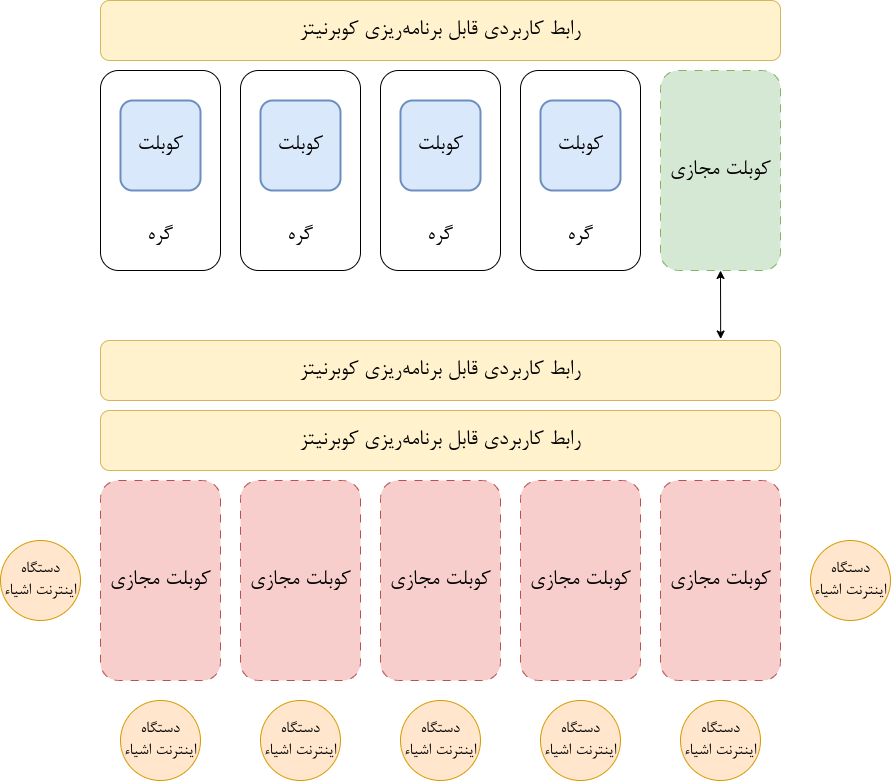
\includegraphics[width=0.8\textwidth]{figs/arch.png}}
        \caption{نمای کلی معماری}
        \label{fig:arch}
    \end{figure}
}
\subsection{پیاده‌سازی تامین‌کننده کوبلت مجازی}
\label{subsec:provider}
\paragraph{}
{
    کوبلت مجازی با در اختیار گذاشتن رابط‌هایی برای برنامه‌نویس، این امکان را می‌دهد که بتوان گره‌های کوبرنیتز با پشتوانه‌های
    سفارشی‌سازی شده داشته باشیم. برای مثال رابط زیر چرخه وجودی یک پاد را نشان می‌دهد. حال با پیاده‌سازی این رابط، ما این امکان
    را داریم که از ساخته‌شدن، بروزرسانی شدن، حذف شدن و حتی تغییر وضعیت‌های پاد‌های مورد نظر خود با خبر شویم.
    \newpage
    \begin{latin}
    \begin{lstlisting}[caption=پاد وجودی چرخه کنترل‌کننده رابط]
        type PodLifecycleHandler interface {
            CreatePod(ctx context.Context, pod *corev1.Pod) error
        
            UpdatePod(ctx context.Context, pod *corev1.Pod) error
        
            DeletePod(ctx context.Context, pod *corev1.Pod) error
        
            GetPod(ctx context.Context, namespace, name string) (*corev1.Pod, error)
        
            GetPodStatus(ctx context.Context, namespace, name string) (*corev1.PodStatus, error)
        
            GetPods(context.Context) ([]*corev1.Pod, error)
        }        
    \end{lstlisting}
    \end{latin}

    پیاده‌سازی این رابط امکان این را می‌دهد که بتوانیم یک پاد بر روی کوبرنیتز اعمال کرده و سپس بوسیله کوبرنیتز فراخوانی شده تا پاد مورد نظر را بسازیم. در  این پروژه یک پاد نقش یک دستگاه اینترنت اشیاء را دارد.
    همچنین برای ارسال وضعیت گره مجازی ساخته شده، نیاز به پیاده‌سازی رابط دیگری داریم.

    \begin{latin}
        \begin{lstlisting}[caption={گره وضعیت کنترل‌کننده رابط}]
            type NodeProvider interface {
                Ping(context.Context) error

                NotifyNodeStatus(ctx context.Context, cb func(*corev1.Node))
            }

        \end{lstlisting}
    \end{latin}

    پیاده‌سازی این رابط باعث می‌شود هنگامی که کد مربوطه در حال اجرا می‌باشد، گره مورد در نظر در خوشه کوبرنیتز بصورت آماده ظاهر شود و اگه این کد متوقف شود، بصورت غیر آماده ظاهر شود.
    بعد از ثبت این دو رابط و انجام چند مرحله دیگر، تامین‌کننده ما آماده استفاده می‌شود و بصورت یک گره در کوبرنیتز ظاهر خواهد شد.
    \begin{figure}[H]
        \center{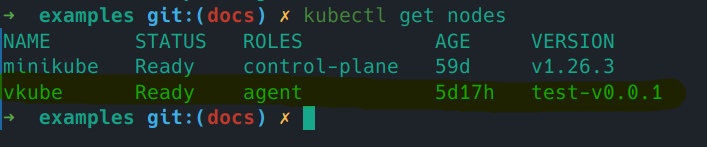
\includegraphics[width=0.8\textwidth]{figs/vkube_node.png}}
        \caption{گره مجازی}
        \label{fig:vkube_node}
    \end{figure}
}
\subsection{رابط برقراری ارتباط با کنترل‌کننده‌ها}
\label{subsec:connector}
\paragraph{}
{
    بعد از اتصال به کوبرنیتز و دریافت درخواست‌ها و بروزرسانی‌ها از سوی این سکو، باید با دستگاه‌های اینترنت اشیاء ارتباط برقرار کرده و وضعیتشان را در اختیار کوبرنیتز قرار دهیم.
    منطق ارتباط با کنترل‌کننده‌های دستگاه‌های اینترنت اشیاء به این صورت است که بصورت مداوم درخواست‌های خاصی به سمت کنترل‌کننده‌ها می‌فرستد تا از وضعیت خود کنترل‌کننده‌ها و همچنین دستگاه‌های اینترنت اشیاء تحت کنترلشان با خبر شود و درصورت نیاز کوبرنیتز را بروزرسانی کند. 
    این درخواست‌ها چیزی نیست جز درخواست‌های قرارداد انتقال فرا متن. همچنین برای اینکه بتوان تعداد زیادی دستگاه‌ اینترنت اشیاء را با یک کنترل‌کننده، کنترل کرد؛ از روش تکرار مقطعی استفاده شده است. این روش به ما کمک می‌کند تا وضعیت دستگاه‌ها را بصورت مقطعی (نه یکجا) دریافت کرده که بتوان در صورت امکان از همزمانی، برای تسریع کار، استفاده کرد.
    \\
    این رابط برای اینکه داده‌های مربوط به وضعیت دستگاه‌ها و کنترل‌کننده‌ها را در اختیار تامین‌کننده قرار دهد، از معماری بازخوانی\footnote{\lr{Callback}} استفاده می‌کند.
}

\subsection{شبیه‌ساز‍}
\label{subsec:simulator}
\paragraph{}
{
    در این پروژه یک شبیه‌ساز هم پیاده‌سازی شده که نقش کنترل‌کننده دستگاه‌های اینترنت اشیاء و همچنین خود این دستگاه‌ها را ایفا می‌کند. این شبیه‌ساز یک خدمت‌دهنده قرارداد انتقال فرامتن می‌باشد که امکانات زیر را هم برای کنترل‌کننده و هم برای دستگاه‌های اینترنت اشیاء فراهم می‌کند:
    \begin{enumerate}
        \item ساخت
        \item ساخت جمعی (برای ارزیابی ساده)
        \item بروزرسانی
        \item حذف
        \item دریافت تکی، همه و مقطعی
    \end{enumerate}
    دستگاه‌های اینترنت اشیاء شبیه‌سازی شده قفل‌های هوشمند یک ساختمان می‌باشند که امکان باز کردن و بستن قفل را دارند.
    \begin{figure}[H]
        \center{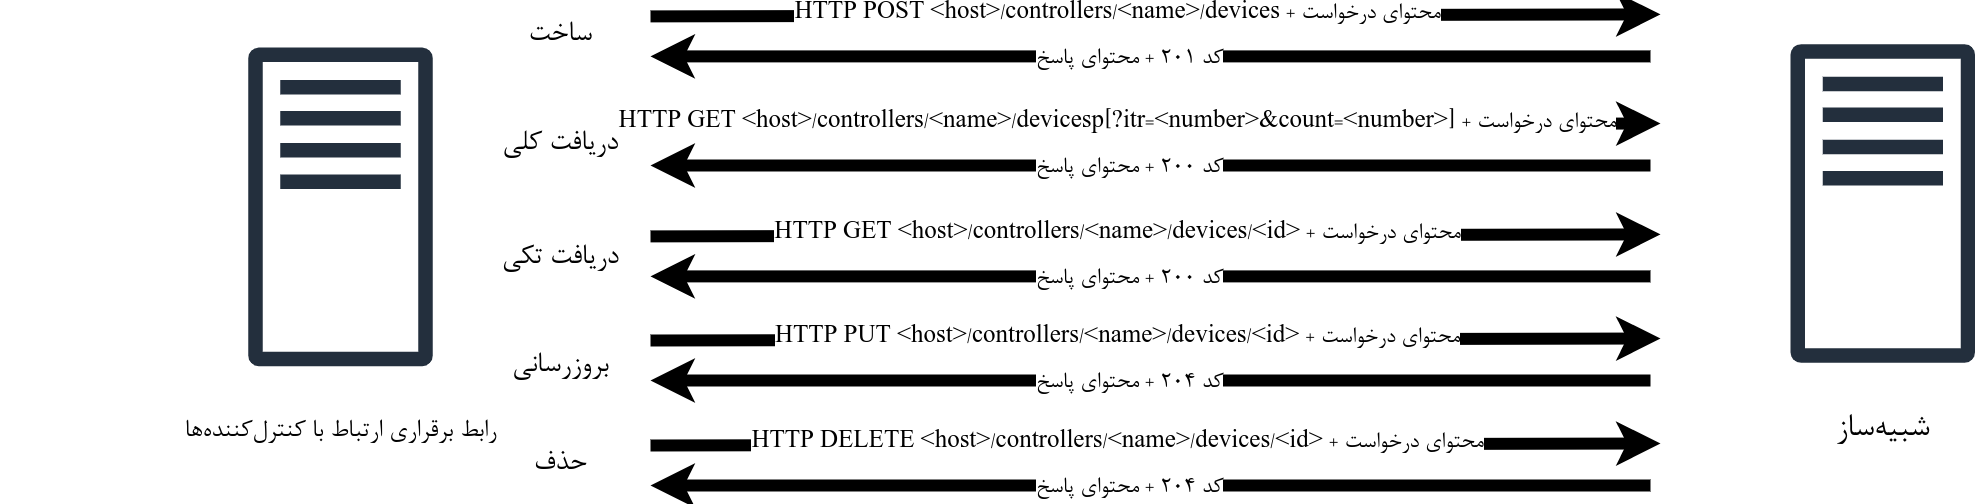
\includegraphics[width=\textwidth]{figs/sim_api.png}}
        \caption{رابط کاربردی قابل برنامه‌نویسی شبیه‌ساز}
        \label{fig:sim_api}
    \end{figure}
}

\subsection{رابط گرافیکی}
\label{subsec:gui}
\paragraph{}
{
    با توجه به اینکه هدف این پروژه امکان‌سنجی و پیاده‌سازی روشی برای پایش دستگاه‌های اینترنت اشیاء بوسیله بستر کوبرنیتز است، اما رابط گرافیکی نیز طراحی شد برای
    نمایش دادن هرچه بهتر اجزای پروژه. این رابط از دو بخش تشکیل شده است.
    \begin{enumerate}
        \item بخشی که با کنترل‌کننده دستگاه‌های اینترنت اشیاء ارتباط دارد و کمک به تسهیل ساخت و نمایش دستگاه‌‌های اینترنت اشیاء می‌کند.
        \item بخش دیگر که با تامین‌کننده در ارتباط است و بصورت مداوم وضعیت گره‌ها و پاد‌های مجازی را بروزرسانی می‌کند.
    \end{enumerate}

    \begin{figure}[H]
        \center{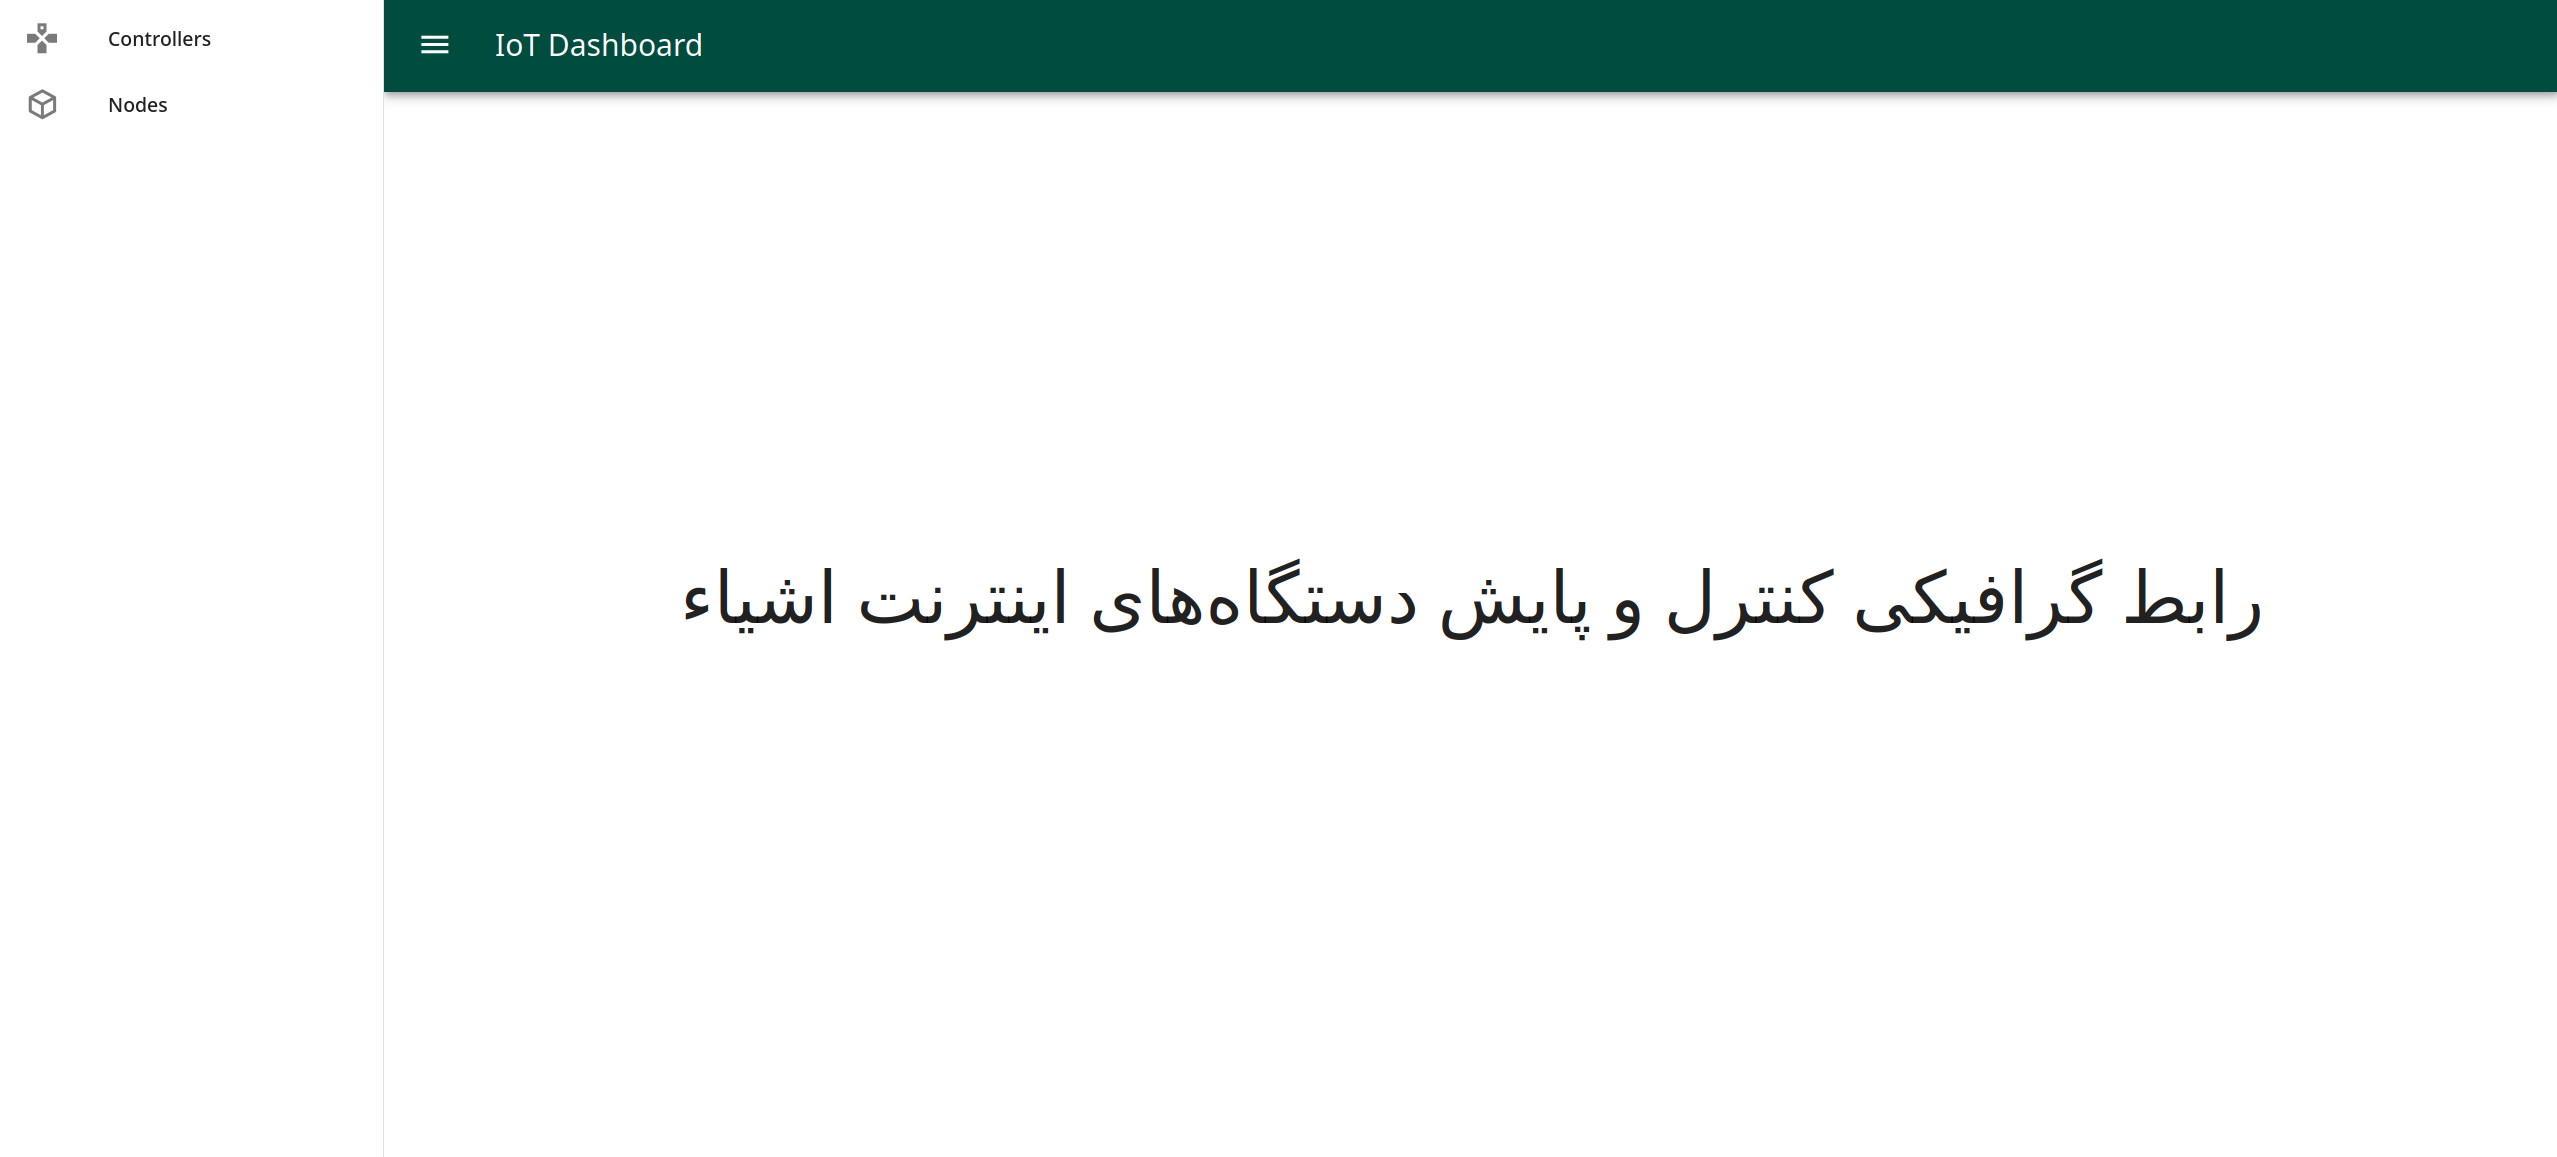
\includegraphics[width=\textwidth]{figs/dash_home.png}}
        \caption{صفحه اصلی رابط گرافیکی}
        \label{fig:dash_home}
    \end{figure}

    \begin{figure}[H]
        \center{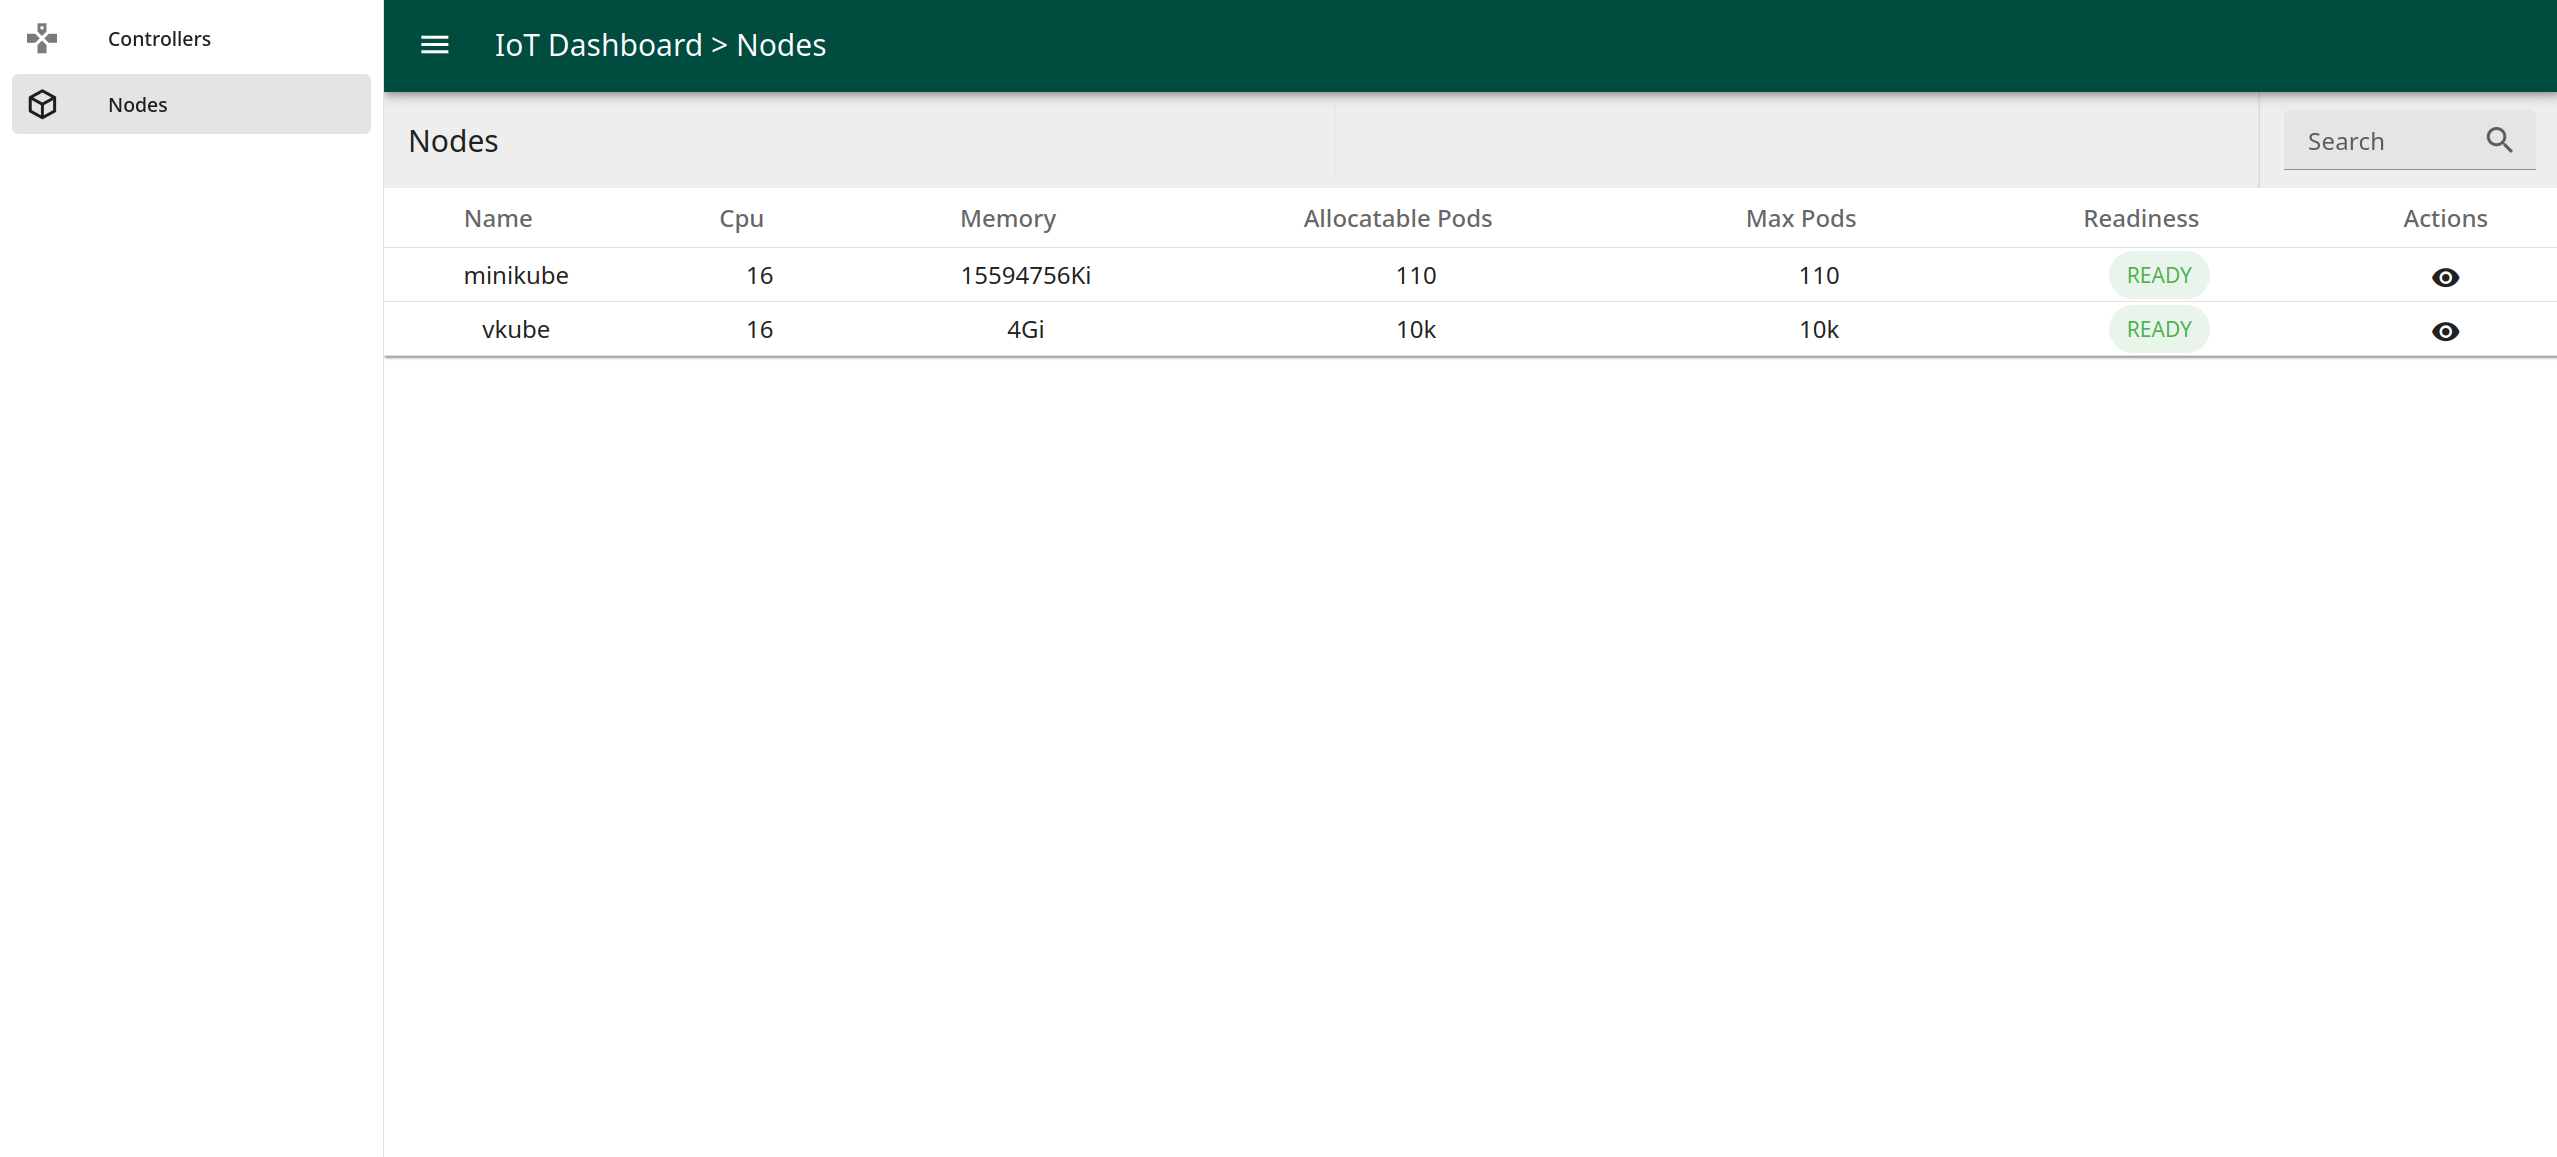
\includegraphics[width=\textwidth]{figs/dash_nodes.png}}
        \caption{صفحه گره‌های کوبرنیتز}
        \label{fig:dash_nodes}
    \end{figure}

    \begin{figure}[H]
        \center{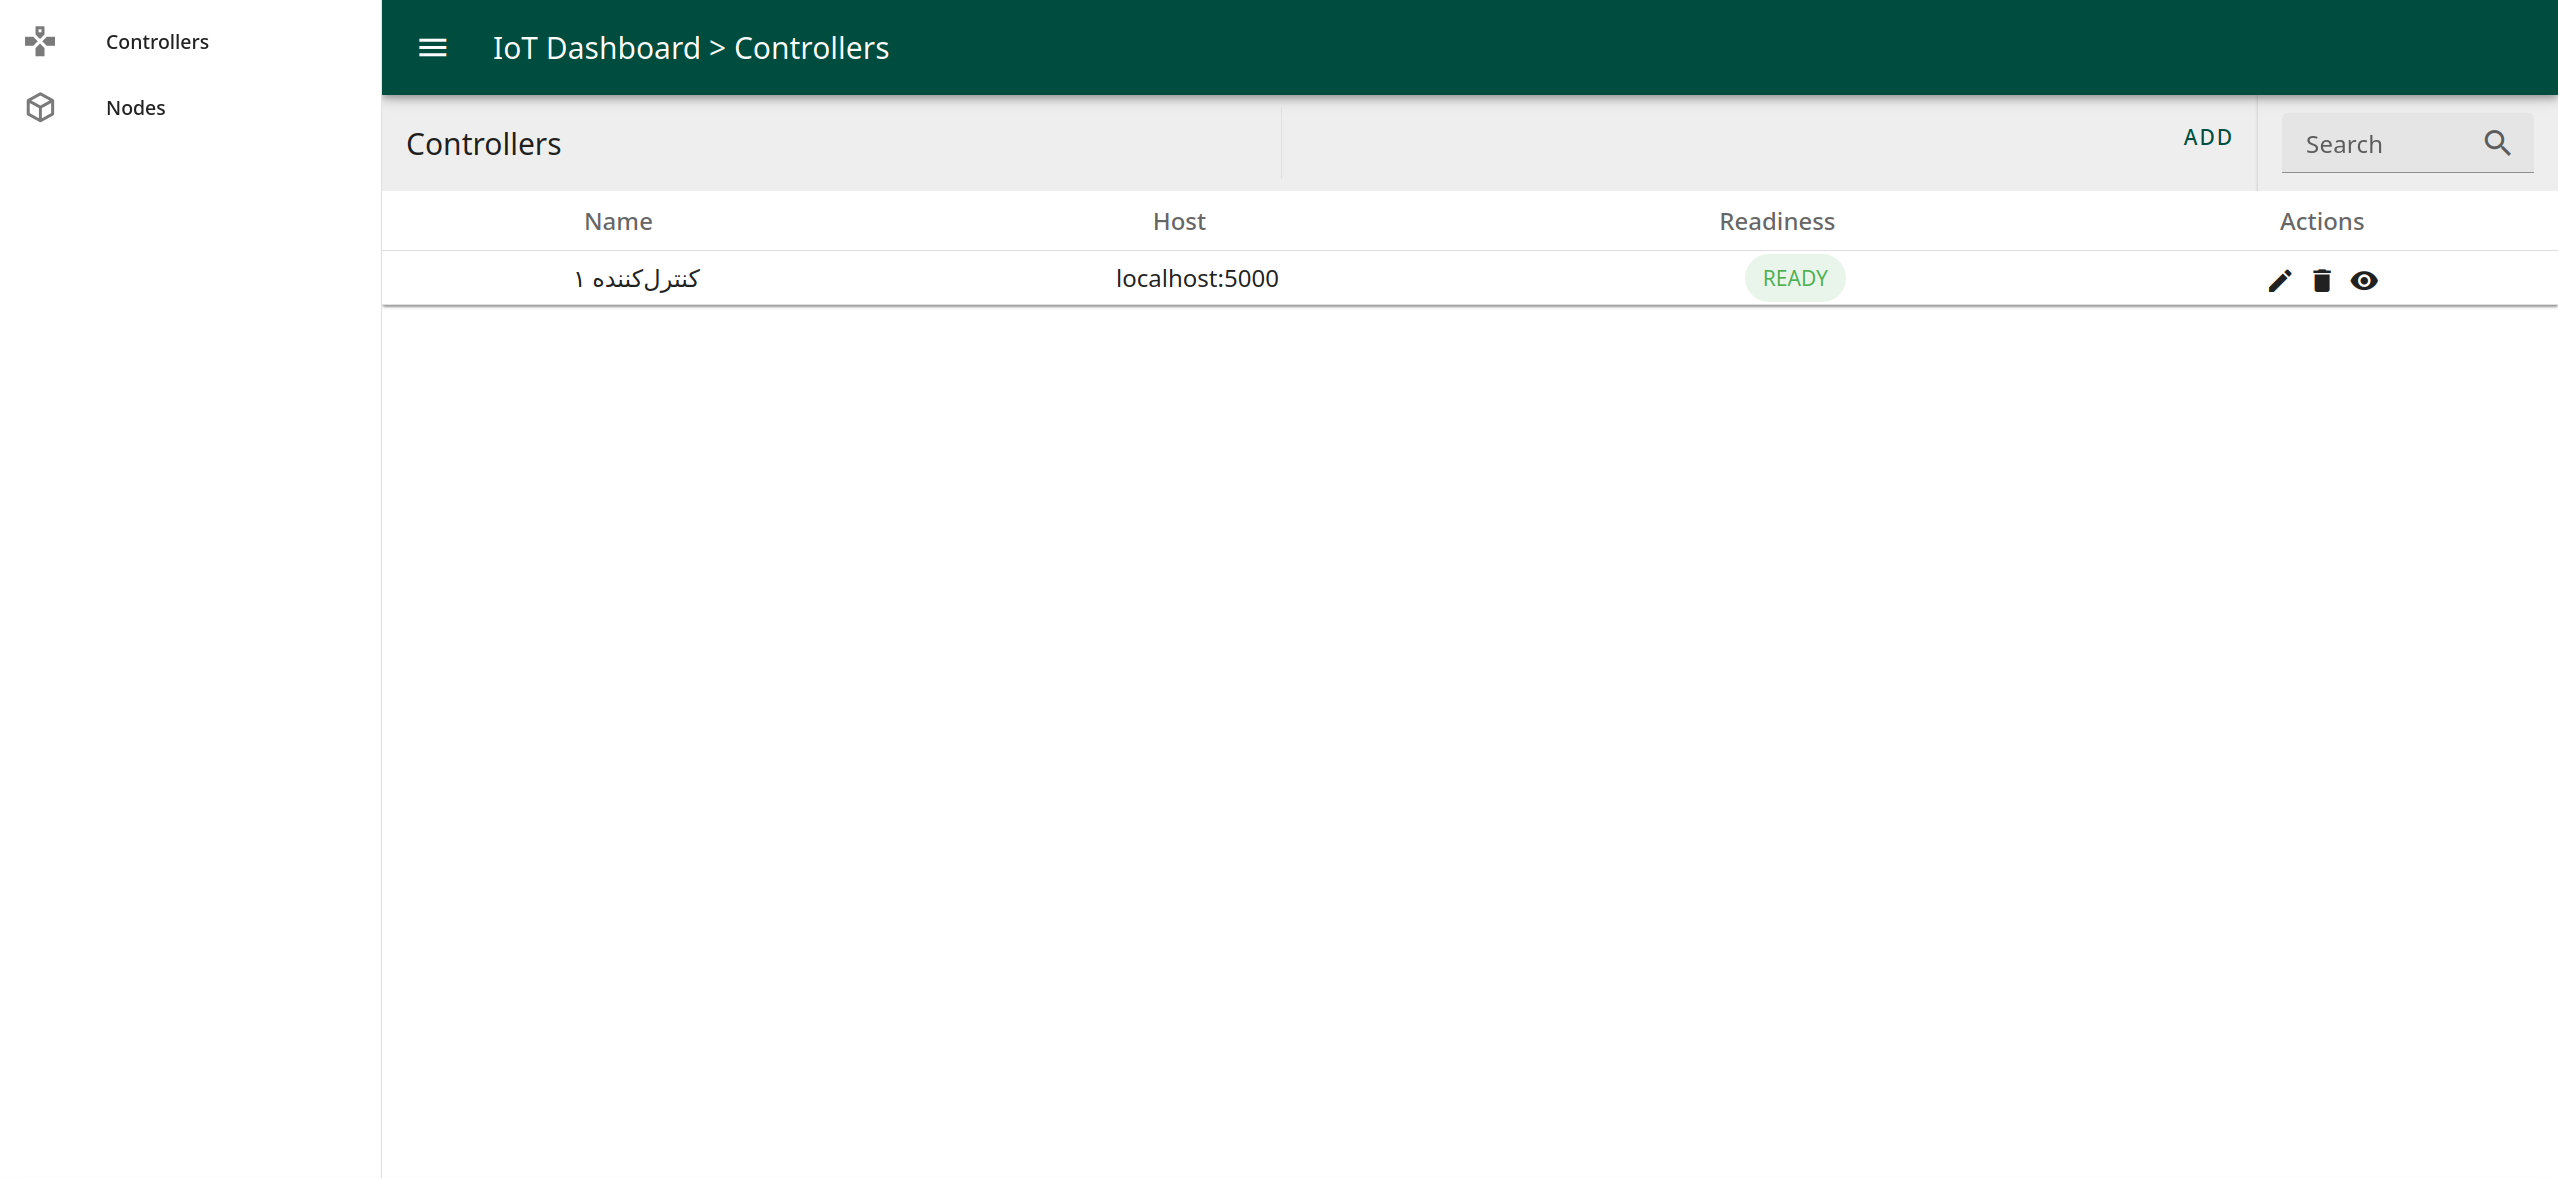
\includegraphics[width=\textwidth]{figs/dash_controllers.png}}
        \caption{صفحه کنترل‌کننده‌های کوبرنیتز کوبرنیتز}
        \label{fig:dash_controllers}
    \end{figure}
}


\section{نحوه کارکرد}
\paragraph{}
{
    ابتدا باید یک مستند پاد که در ذیل آمده مهیا کرده و در کوبرنیتز اعمال کنیم. بعد از اعمال این مستند،
    کوبرنیتز تامین‌کننده را از ایجاد این مستند با خبر می‌کند. حال تامین کننده با بازفراخوانی رابط کنترل‌کننده‌ها
    منجر به شروع دریافت وضعیت این دستگاه اینترنت اشیاء بصورت مداوم از کنترل‌کننده تعریف شده در مستند می‌شود.
    بنابراین رابط کنترل‌کننده‌ها بصورت مداوم با رابط کاربردی قابل برنامه‌نویسی شبیه‌ساز ارتباط گرفته و وضعیت دستگاه‌ها
    را بروزرسانی می‌کند.
    \newpage
    \begin{latin}
        \begin{lstlisting}[caption=کوبرنیتز در پاد ساخت مستند]
            apiVersion: v1
            kind: Pod
            metadata:
              name: lock-main
              annotations:
                controllerName: "controller1" 
                controllerAddress: "localhost:5000"
            spec:
              containers:
              # this is so that kubernetes validation will pass
                - image: doesntmatter/smart_lock
                  name: lock1
              dnsPolicy: ClusterFirst
              nodeSelector:
                kubernetes.io/role: agent
                kubernetes.io/os: linux
                type: virtual-kubelet
              tolerations:
              # this will target Virtual Kubelets nodes only
                - key: itzloop.dev/virtual-kubelet
                  operator: Exists
        \end{lstlisting}
    \end{latin}
    \newpage
    قبل از اعمال مستند بالا، از طریق رابط گرافیکی در  شبیه‌ساز چهار دستگاه ساخته که در شکل زیر مشاهده می‌کنید.
    \begin{figure}[H]
        \center{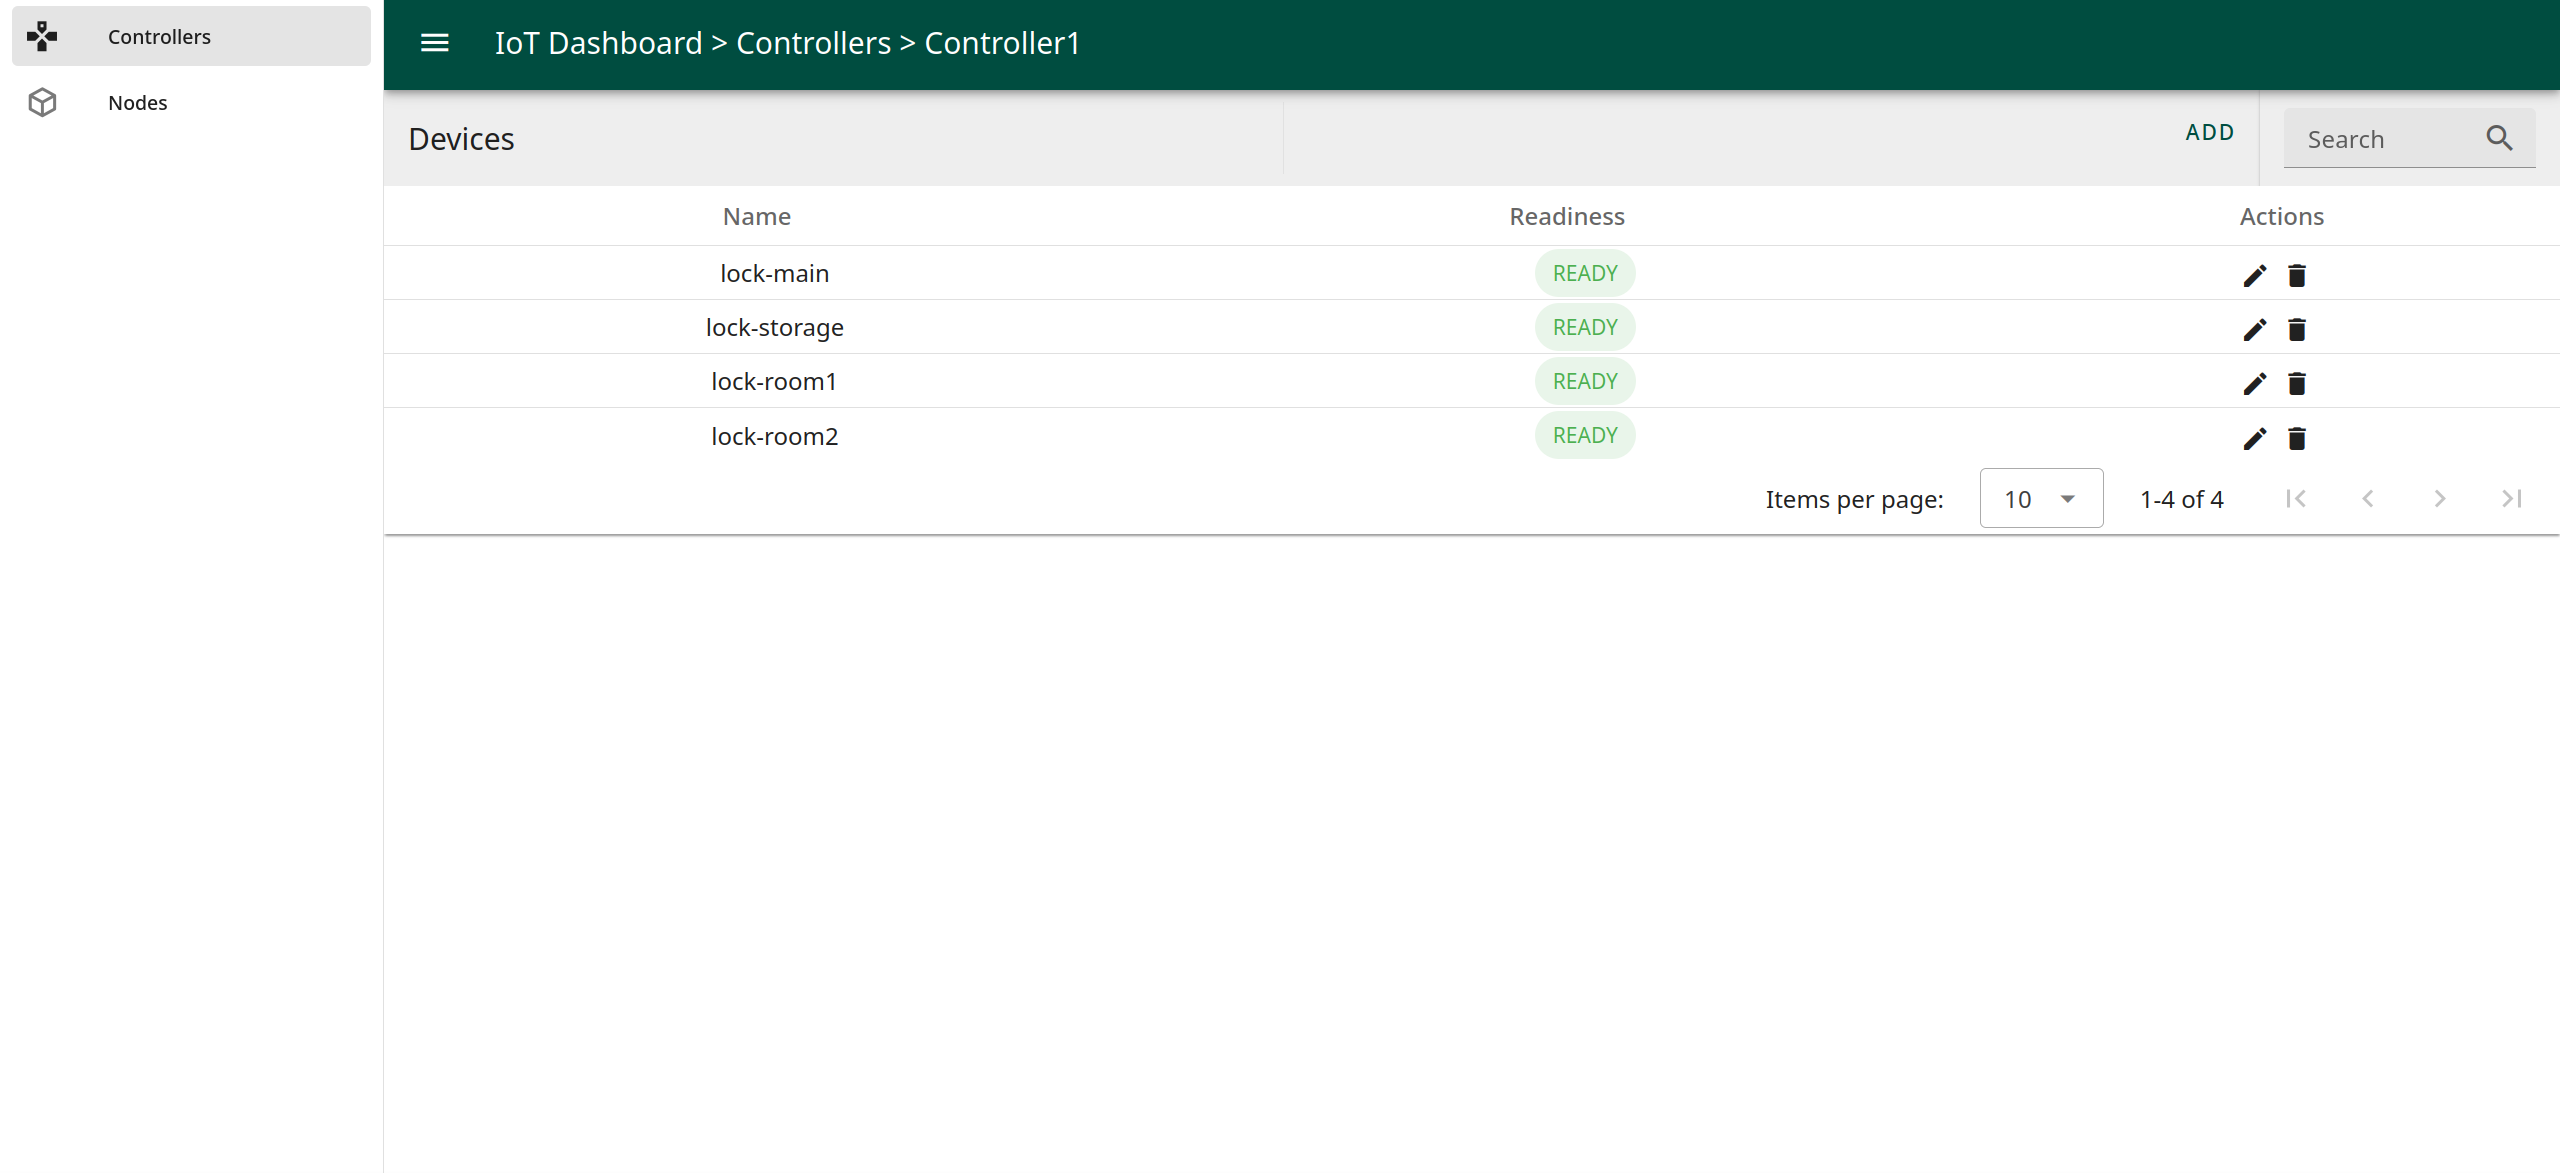
\includegraphics[width=\textwidth]{figs/dash_devices.png}}
        \caption{دستگاه‌های اینترنت اشیاء ساخته شده در شبیه‌ساز}
        \label{fig:dash_devices}
    \end{figure}
    در ادامه مستند پاد را اعمال می‌کنیم. همانطور که در مستند آماده است فقط یکی از این دستگاه‌ها یعنی قفل مرکزی\footnote{lock-main} را از طریق کوبرنیتز رصد می‌کنیم. بعد از اعمال این مستند پاد‌های کوبرنیتز را مشاهده‌ کرده که ابتده در وضعیت عدم آمادگی\footnote{\lr{Not-Ready}} می‌باشند.
    \begin{figure}[H]
        \center{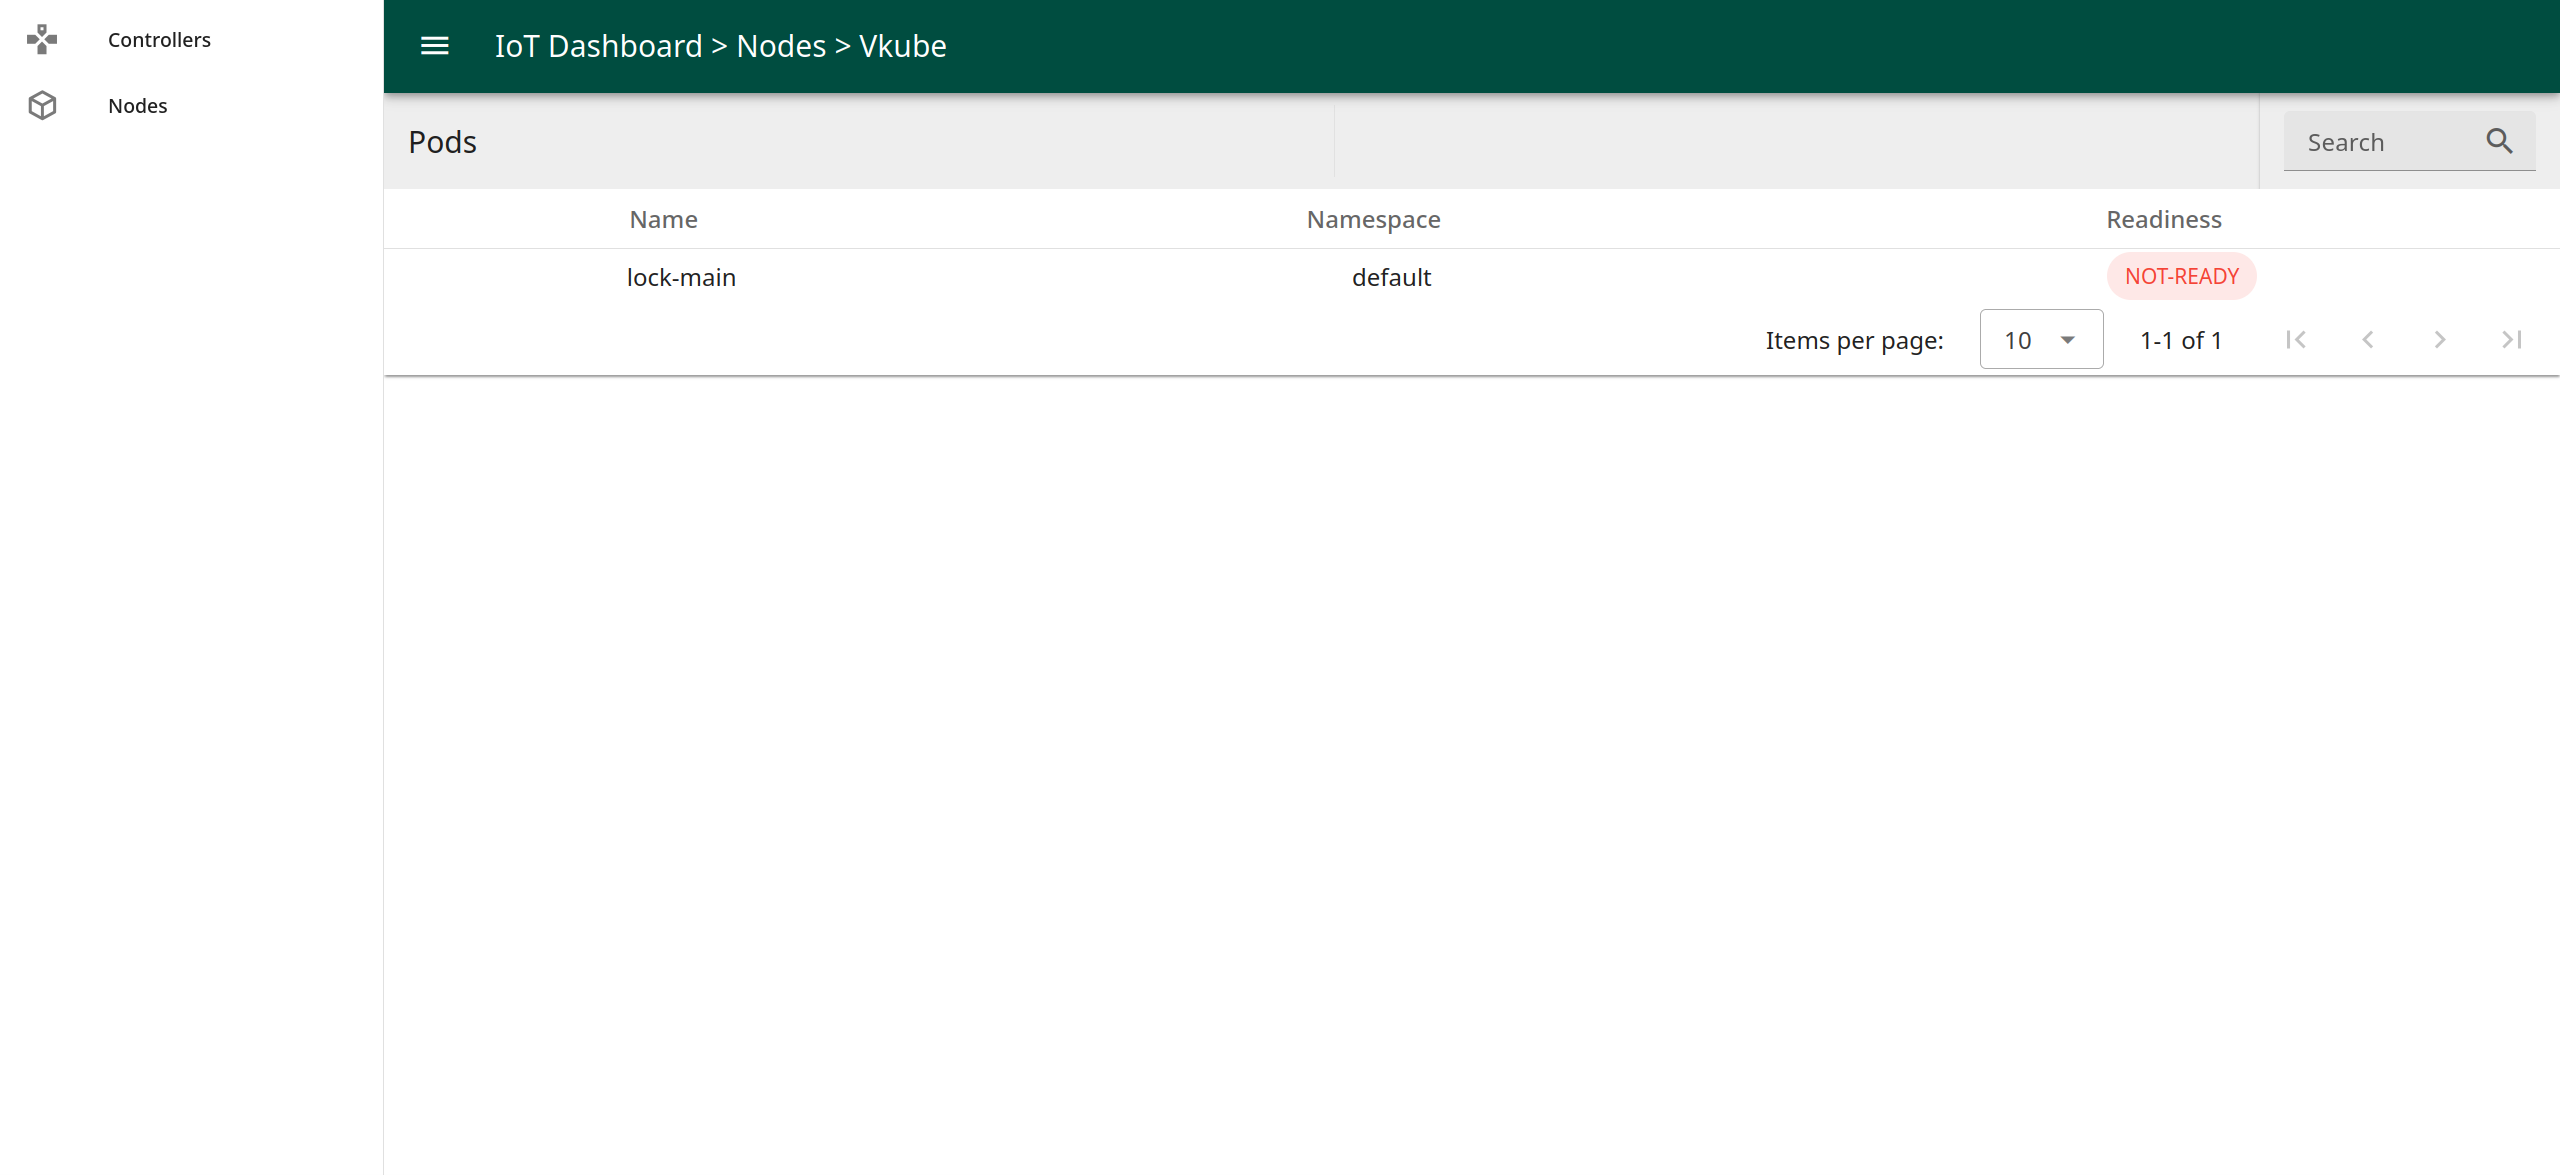
\includegraphics[width=\textwidth]{figs/dash_pod_lock_main_not_ready.png}}
        \caption{پاد ساخته شده از روی مستند در وضعیت عدم آمادگی}
        \label{fig:dash_pod_lock_main_not_ready}
    \end{figure}
    پس از گذر مدتی (مدت زمانی که طول می‌کشد رابط ارتباط با کنترل‌کننده‌ها وضعیت قفل مرکزی را از شبیه‌ساز دریافت کند) خواهیم دید که پاد مورد نظر در کوبرنیتز به وضعیت آماده\footnote{\lr{Ready}} در می‌آید.
    \begin{figure}[H]
        \center{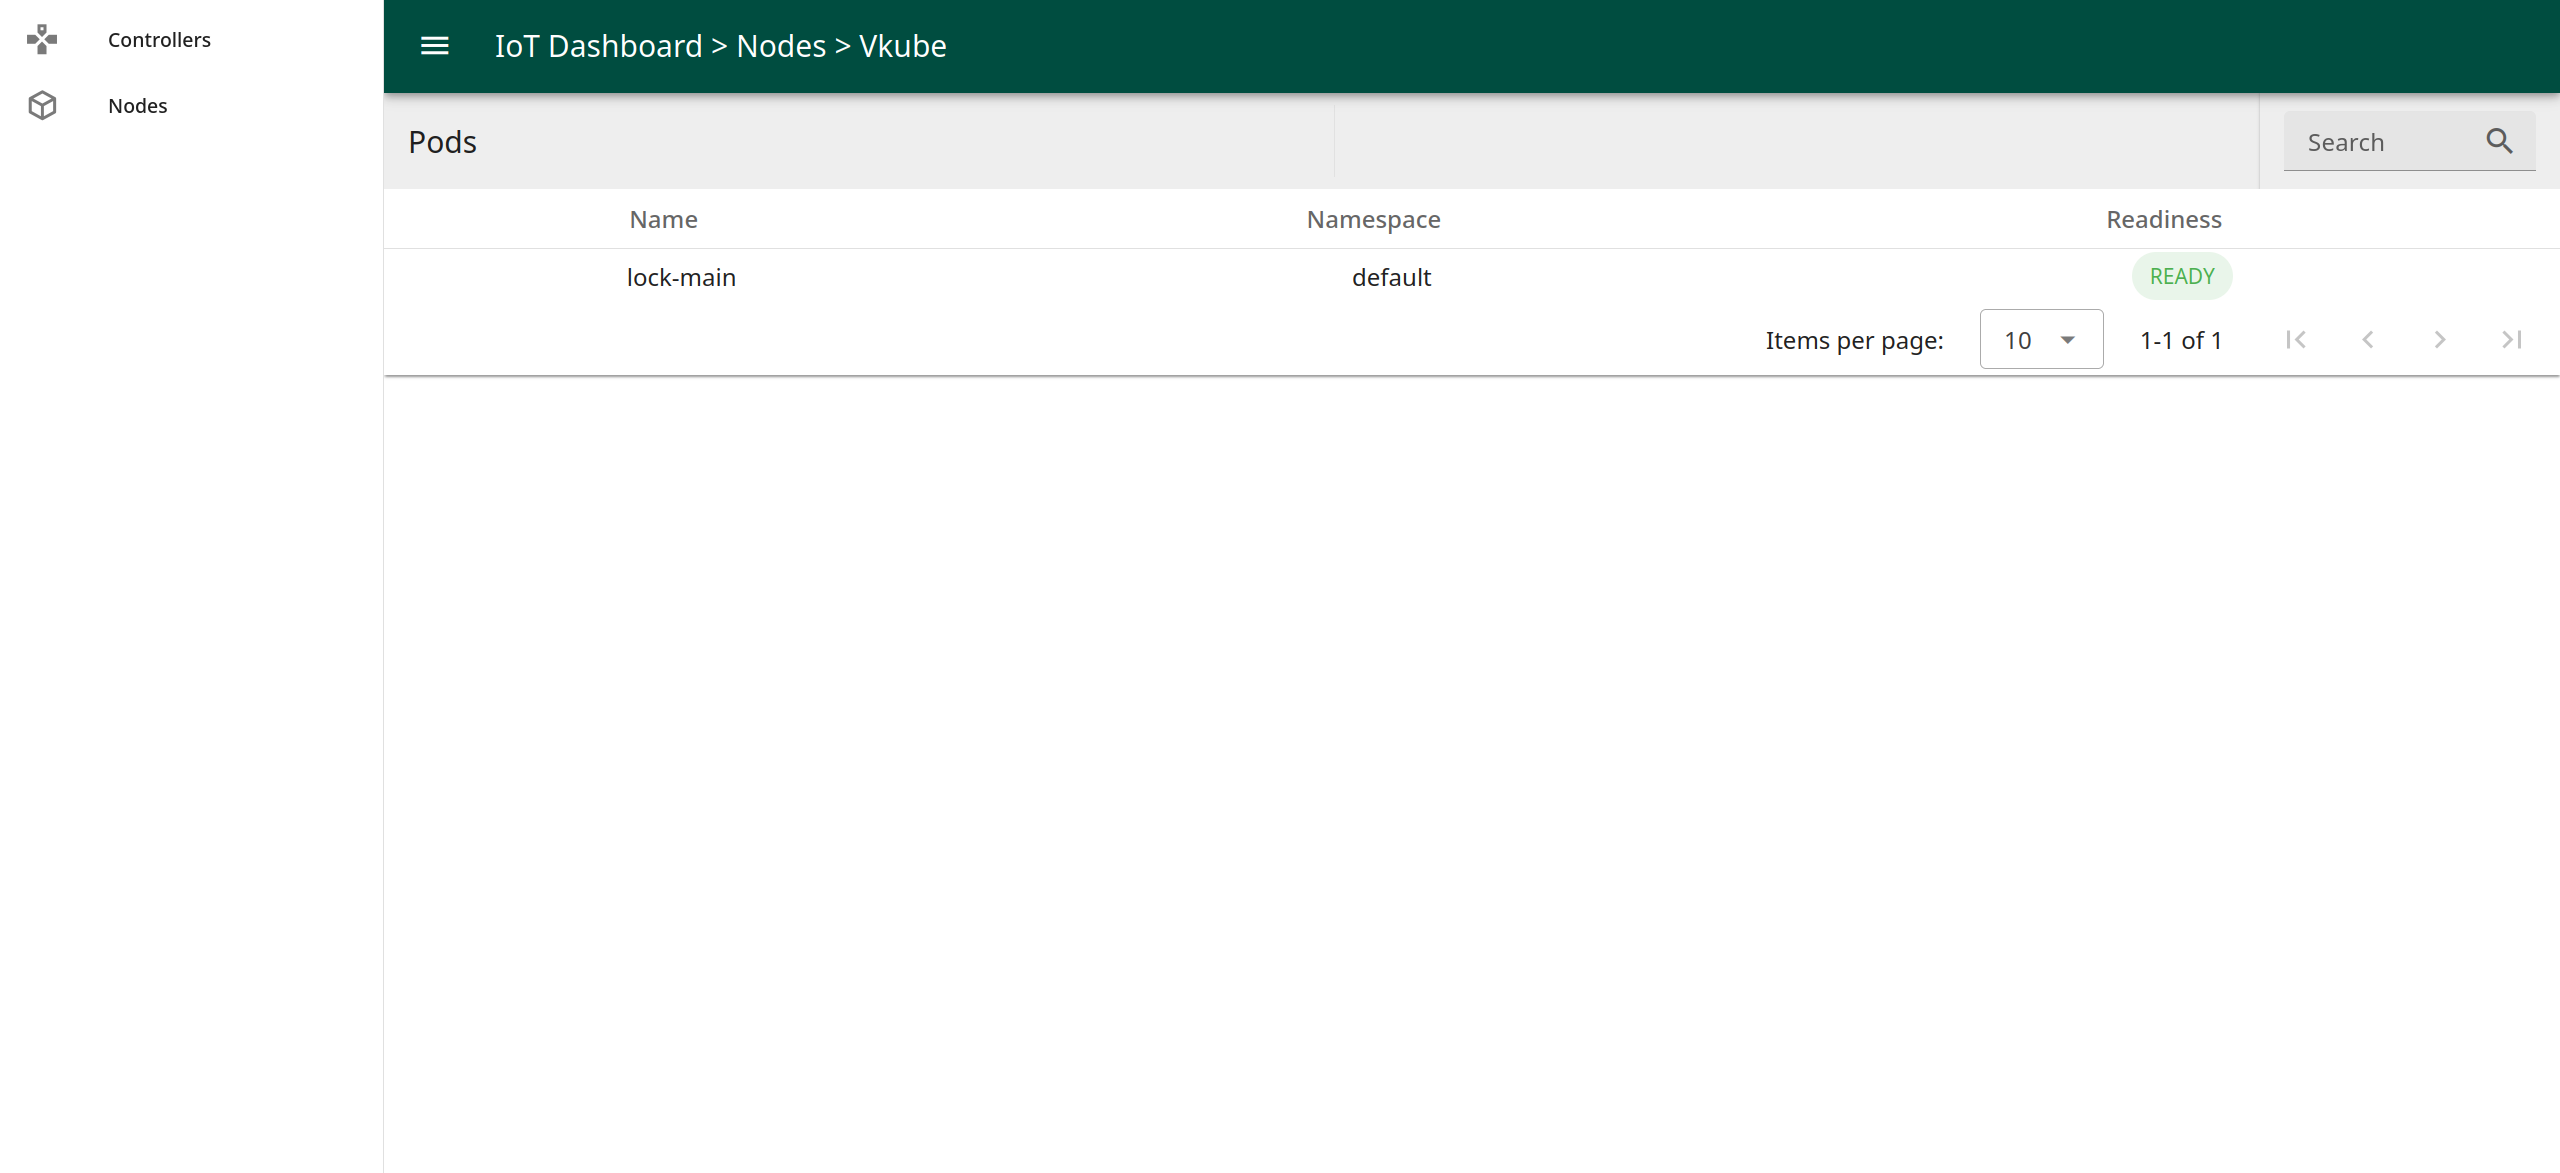
\includegraphics[width=\textwidth]{figs/dash_pod_lock_main_ready.png}}
        \caption{پاد ساخته شده از روی مستند در وضعیت آماده}
        \label{fig:dash_pod_lock_main_ready}
    \end{figure}

    حال اگر با استفاده از رابط گرافیکی، وضعیت قفل مرکزی در شبیه‌ساز را به وضعیت عدم آمادگی تغییر دهیم خواهیم دید که بعد از مدتی وضعیت پاد نیز تغییر می‌کند.
    \begin{figure}[H]
        \center{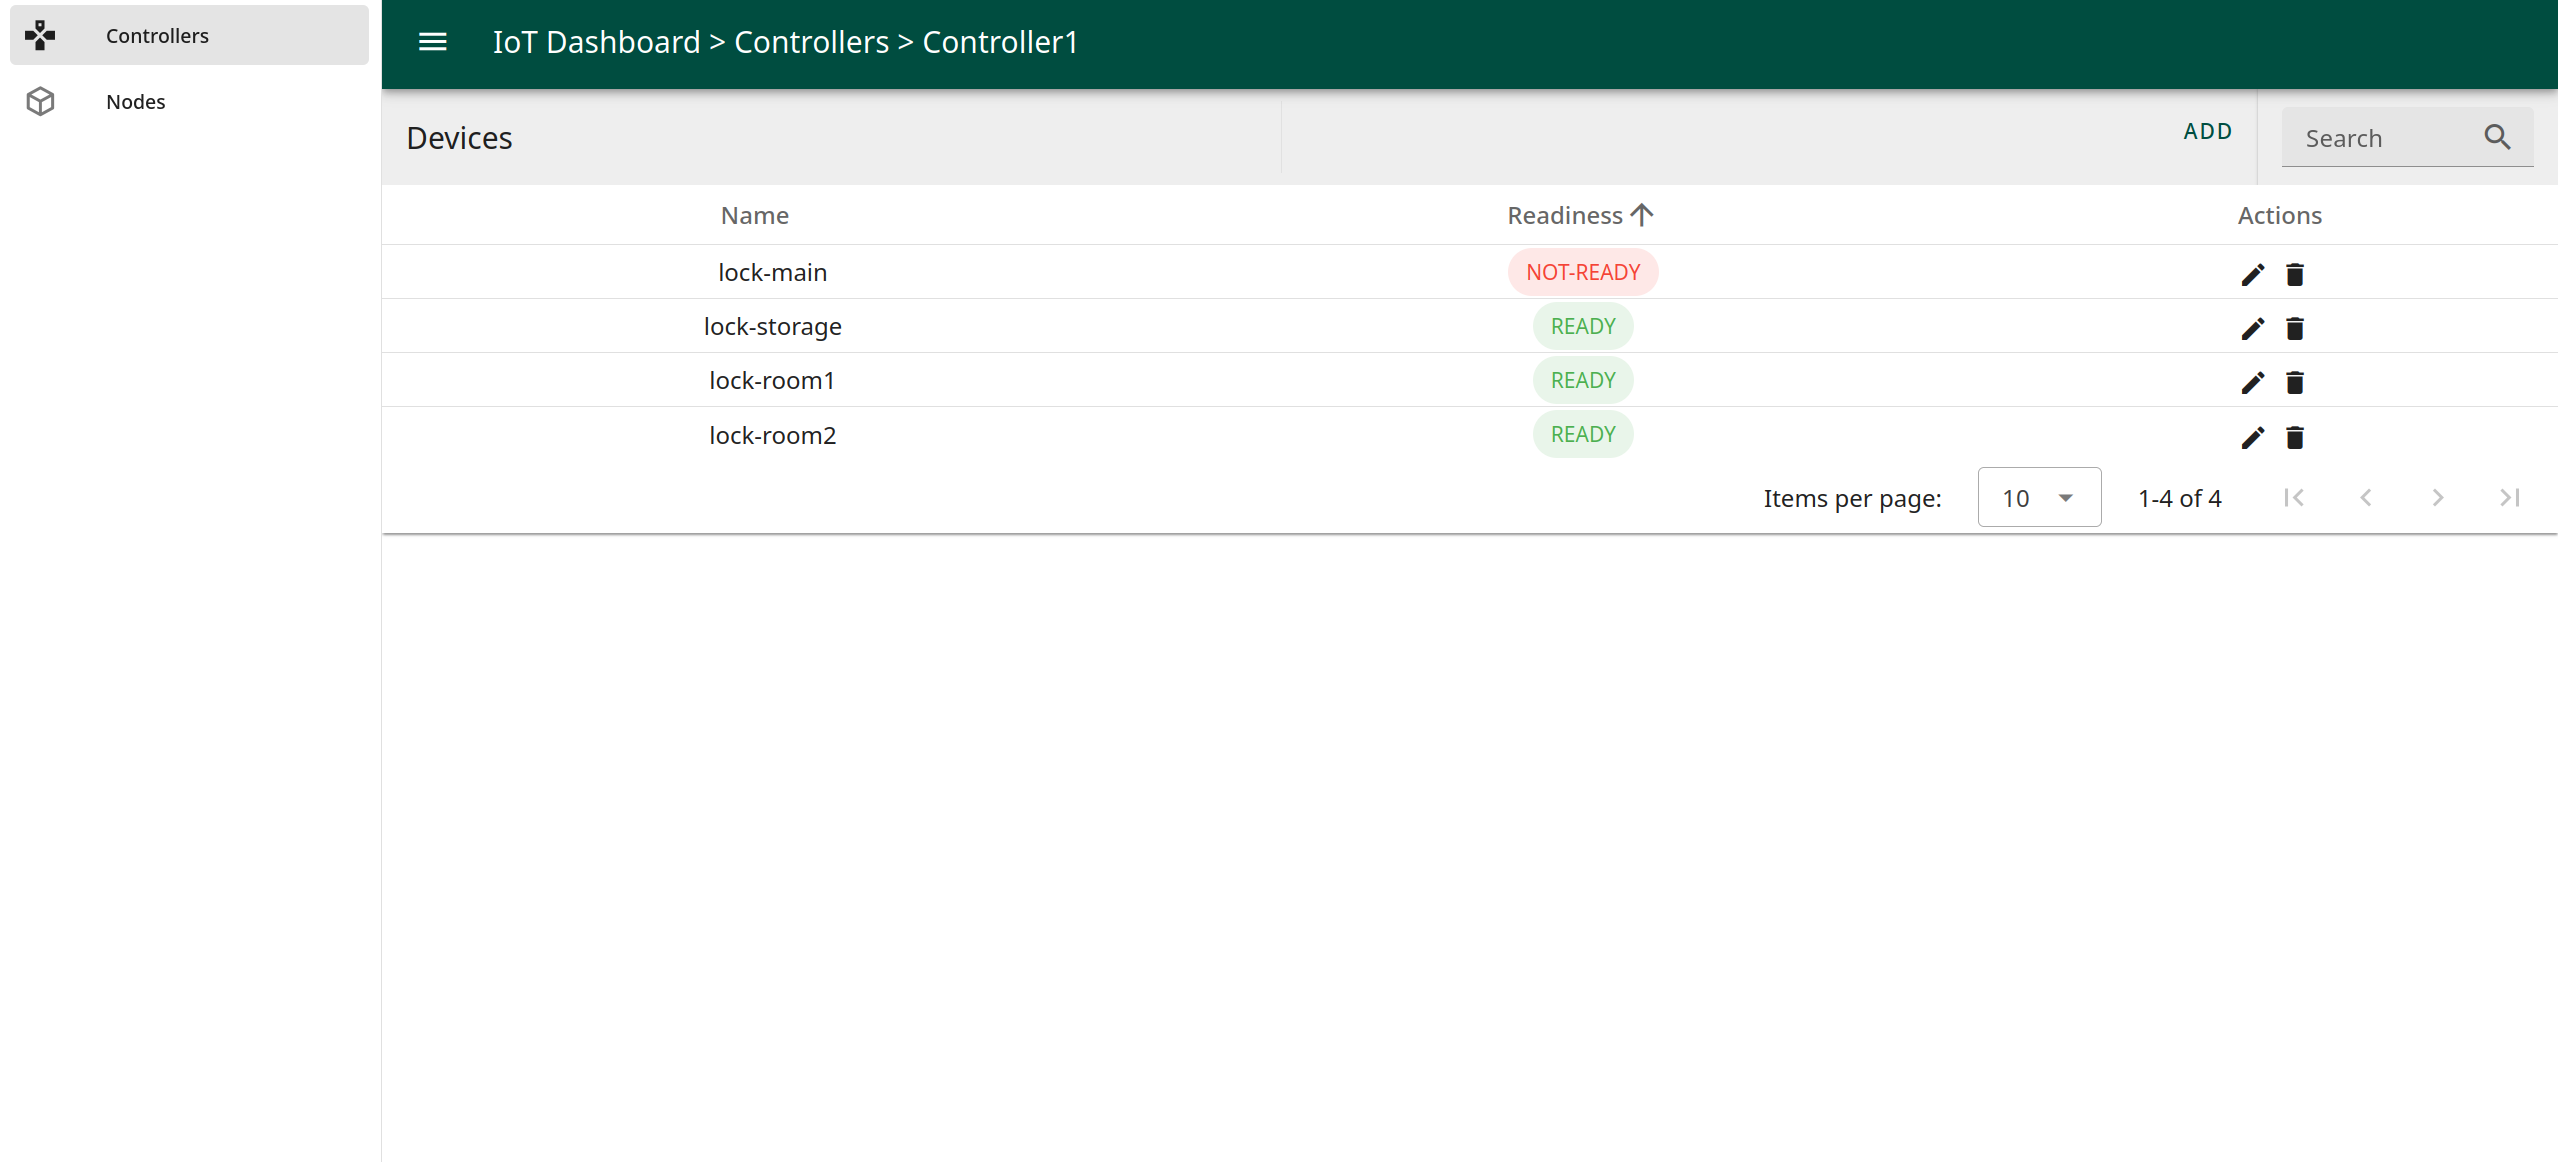
\includegraphics[width=\textwidth]{figs/dash_lock_main_change_readiness.png}}
        \caption{تغییر وضعیت قفل مرکزی در رابط گرافیکی}
        \label{fig:dash_lock_main_change_readiness}
    \end{figure}

    \begin{figure}[H]
        \center{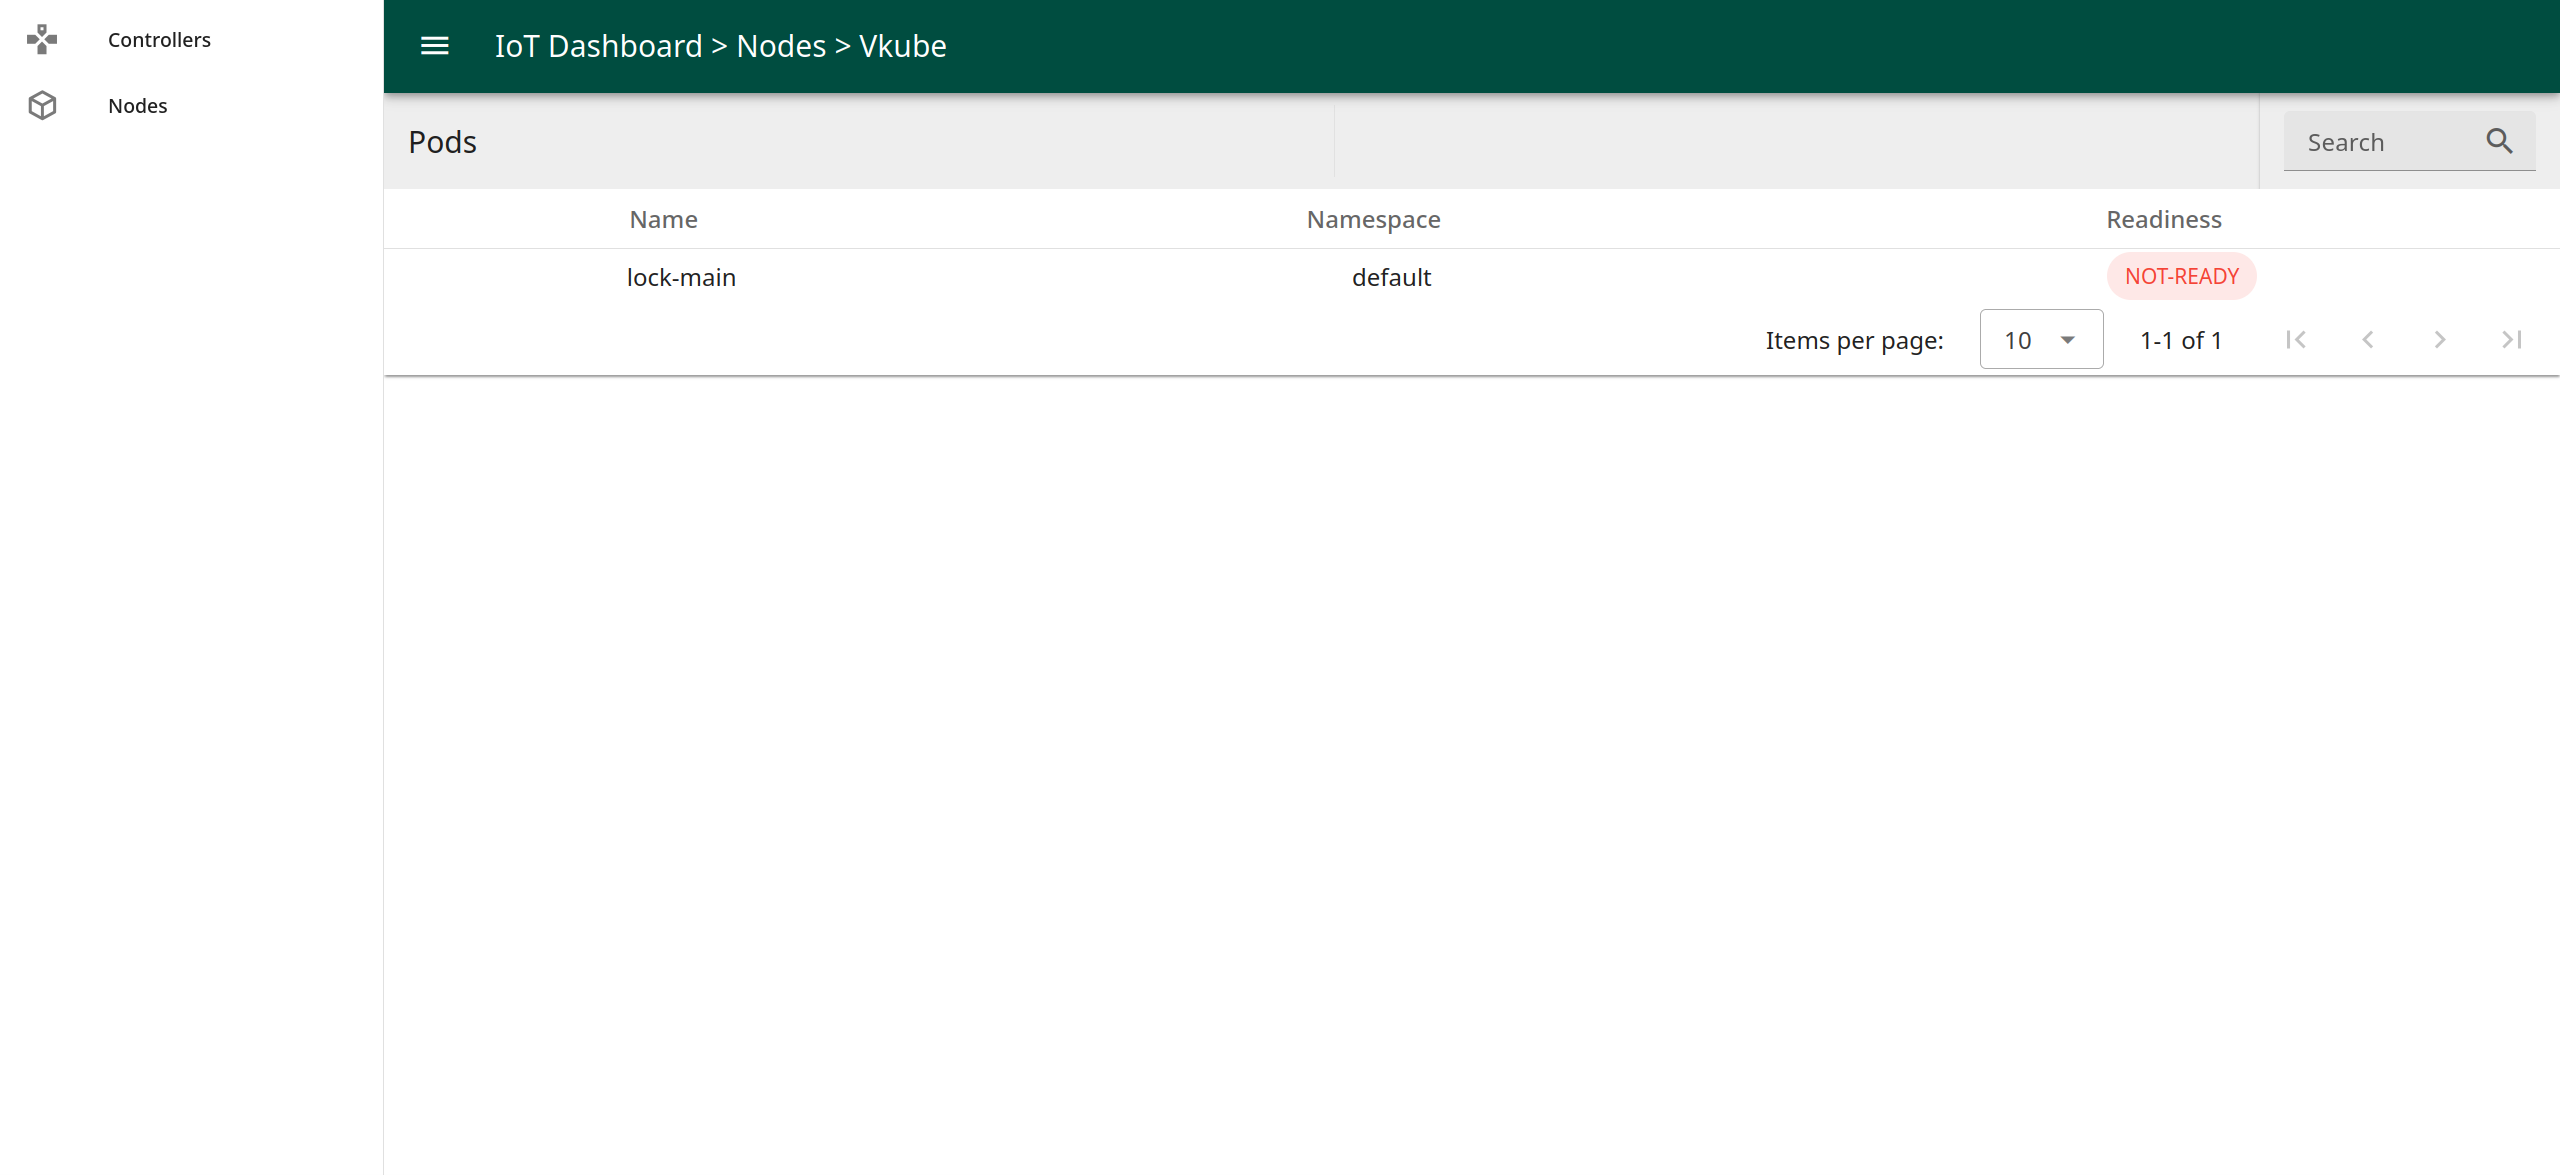
\includegraphics[width=\textwidth]{figs/dash_pod_lock_main_not_ready.png}}
        \caption{تغییر وضعیت پاد بدلیل تغییر وضعیت قفل مرکزی}
        \label{fig:dash_pod_lock_main_change readiness}
    \end{figure}
}

% \section{مقدمه}
% \paragraph{}{
%     هدف از این پژوهش انتشار روشی برای تولید پاسخ‌ها به صورت جمله است. برای این 
%     مورد، از شبکه‌های از پیش‌آموزش داده شده استفاده شده است. از 
%     \lr{LXMERT} \cite{tan-bansal-2019-lxmert}
%     به عنواان یک معماری دو‌جریان و از 
%     \lr{VisualBERT} \cite{li-etal-2020-bert-vision}
%     به عنوان یک معماری تک‌جریان بهره‌برداری شده است. 
% }


% % \vspace{15pt}

% \section{
%   معماری سیستم
%  }
% \paragraph{}{
%     برای حل این مسسله از معماری کدگذار-کدگشا استفاده شده‌است به گونه‌ای 
%     که از یک شبکه از پیش آموزش داده‌شده به عنوان کدگذار و از معماری‌های متفاوتی 
%     به عنوان کدگشا استفاده شده است. 
    
% }

% % \newpage

% % \vspace*{20pt}


% \begin{figure}[H]
%     % \center{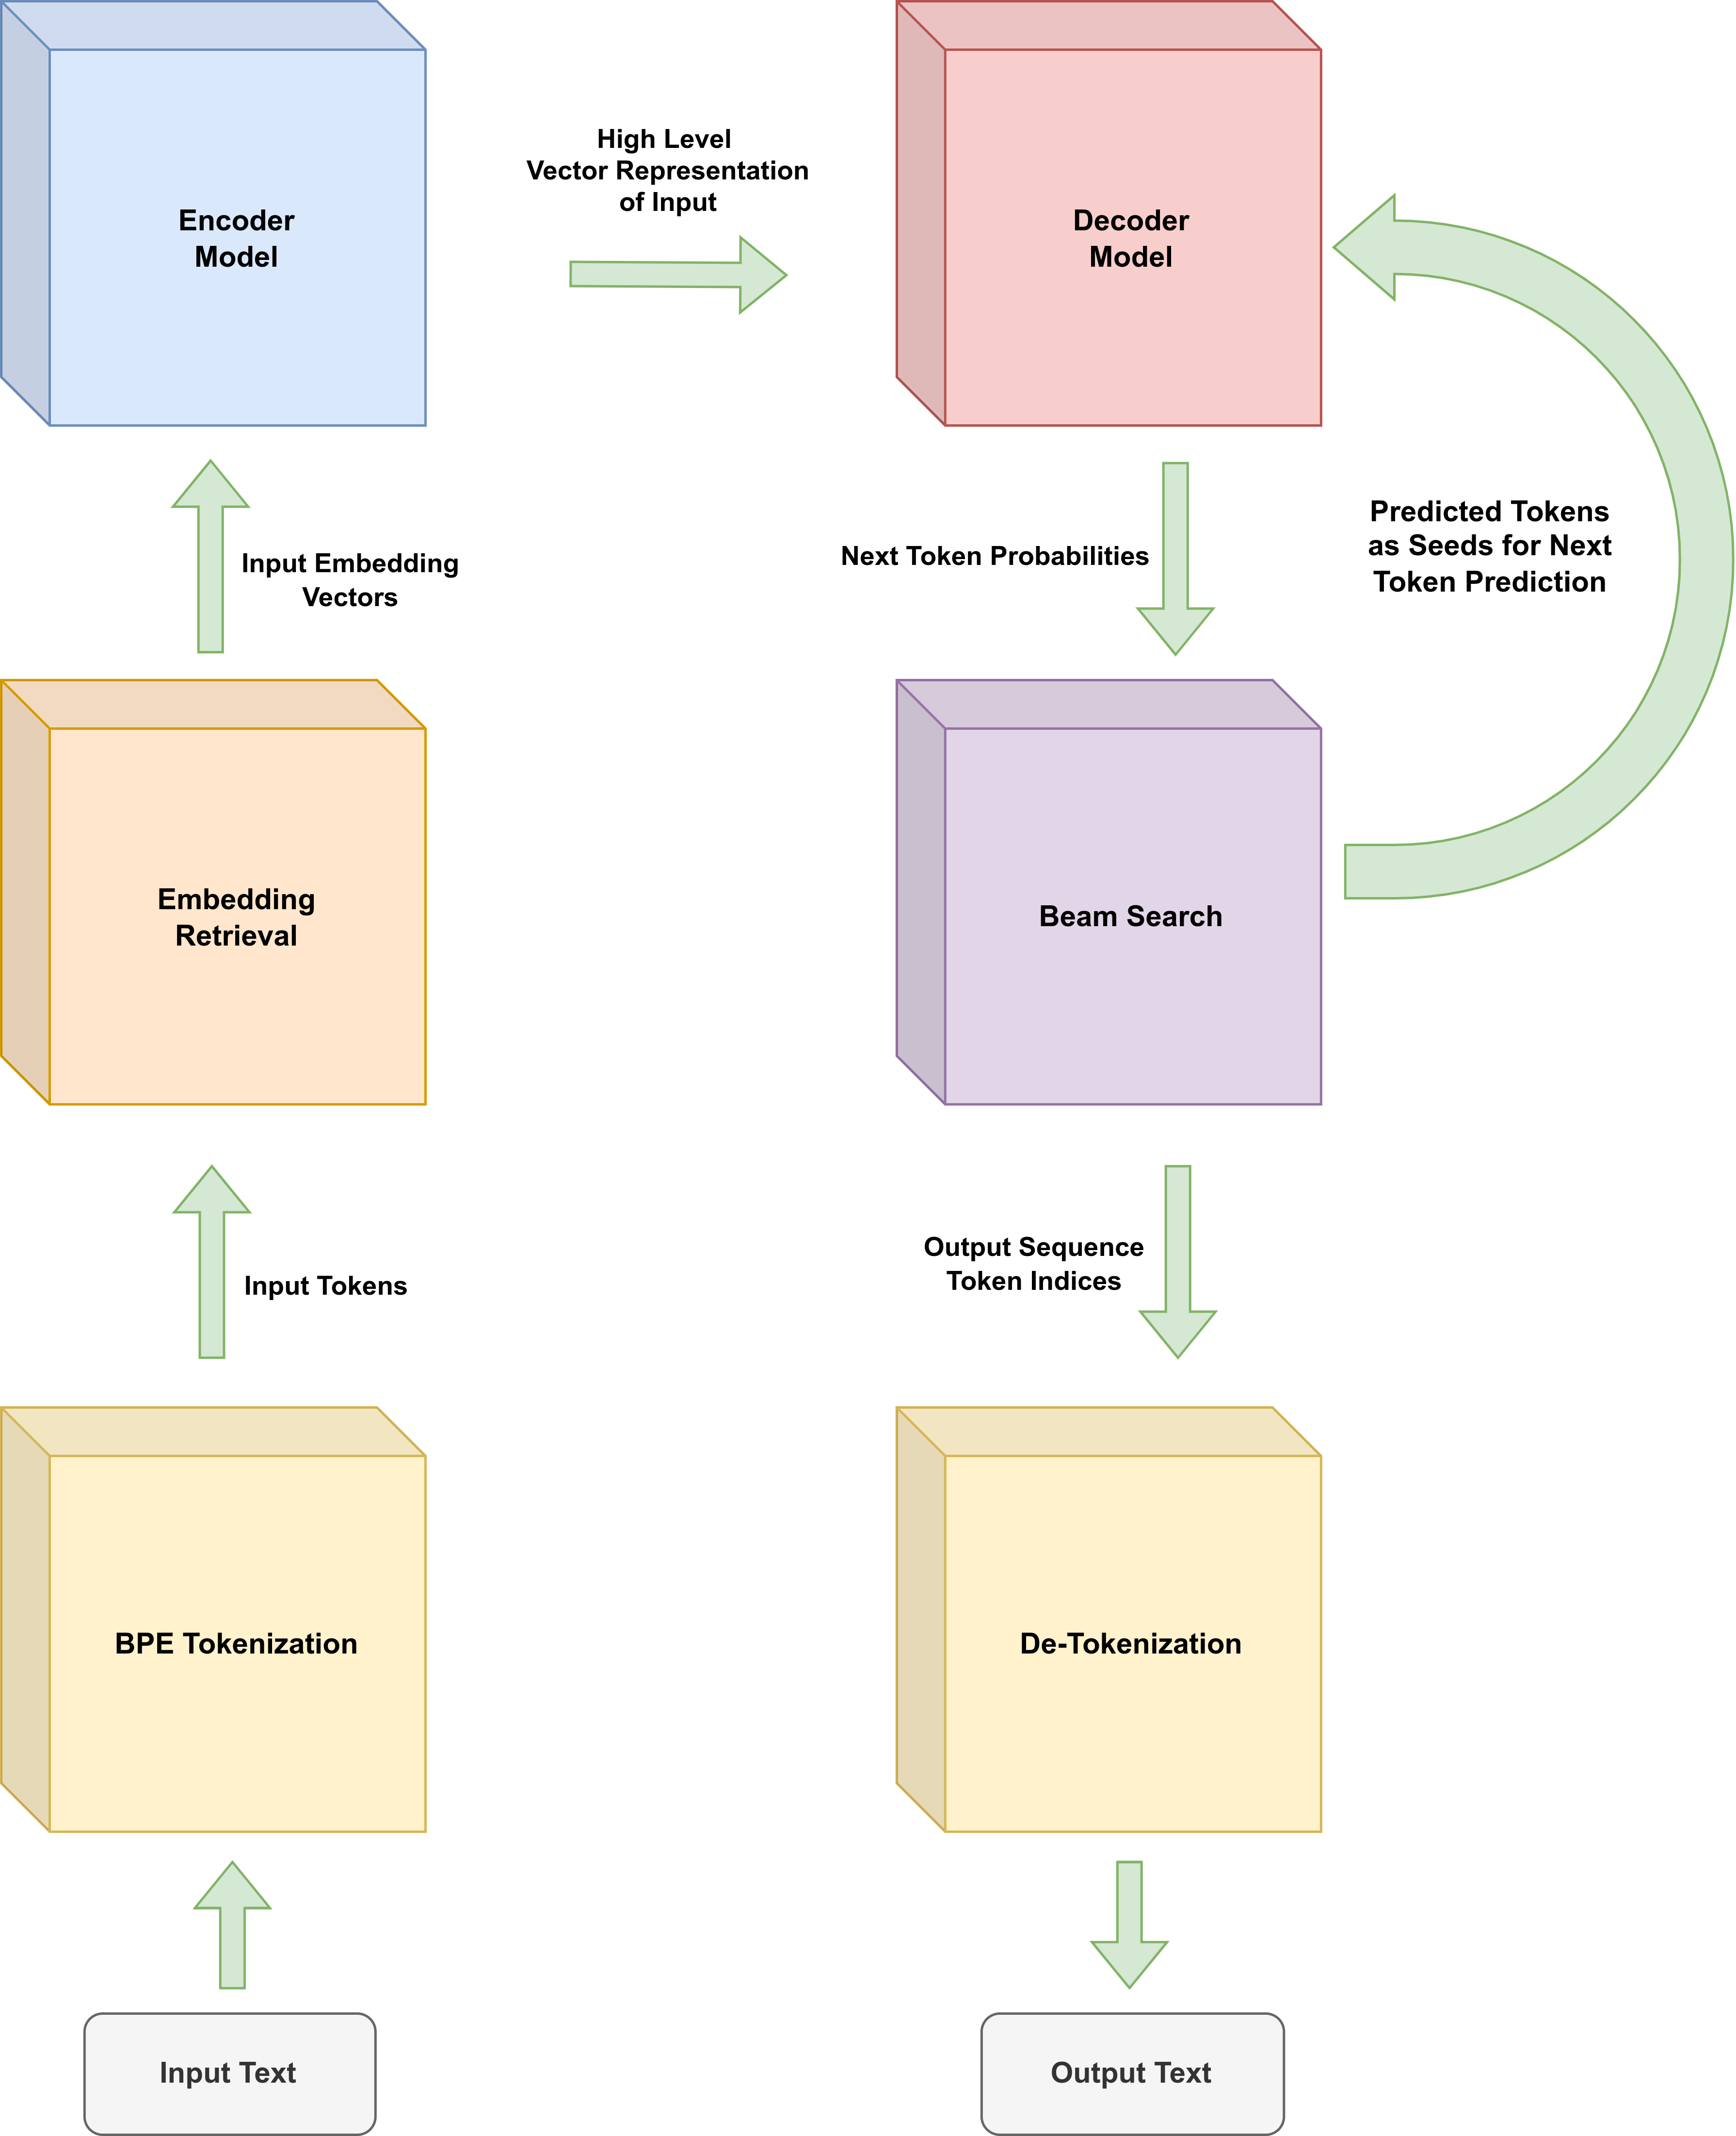
\includegraphics[width=1\textwidth]{figs/overview.png}}
%     \center{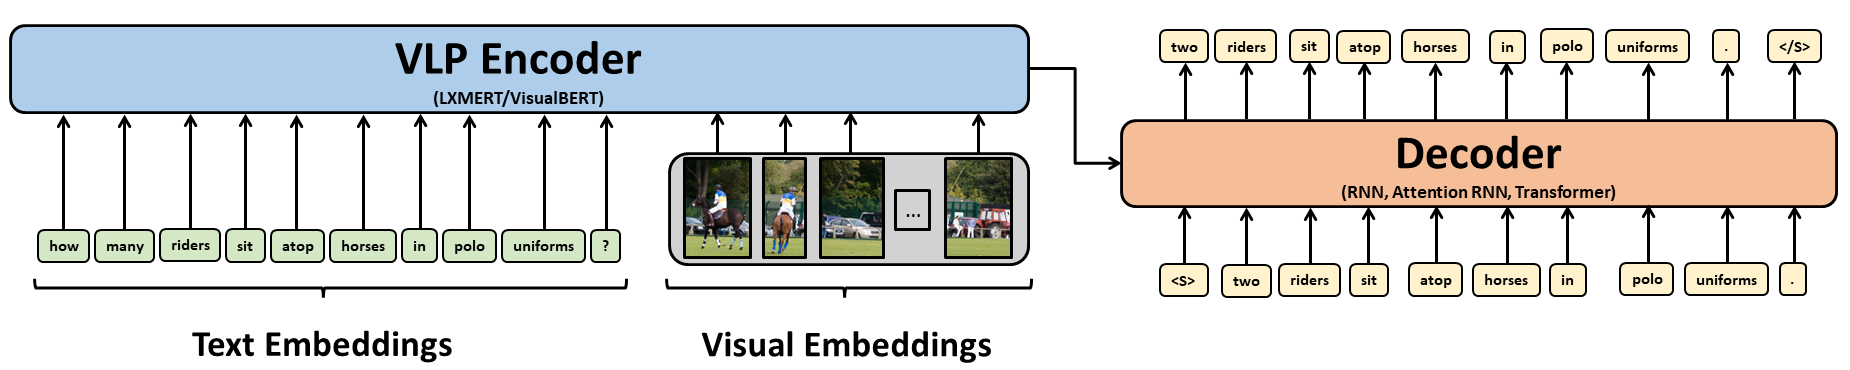
\includegraphics[width=1\textwidth]{figs/model architecture.png}}
%     \caption{شمای کلی سیستم پرسش‌و‌پاسخ تصویری}
%     \label{fig:overview}
% \end{figure}

% \newpage

% \section{
%   ورودی اولیه و خروجی نهایی
%  }

% \paragraph{}{
%     در ورودی سیستم باید بتوانیم تصویر و متن را به سیستم ورودی بدهیم. برای 
%     انجام این عمل باید هر دو بخش متن  و تصاویر را به بردار‌های ویژگی تبدیل کنیم. 
    
%     \begin{enumerate}
%         \item \textbf{بردارهای متن:}
%                 برای پردازش دقیق پرسش‌ها، لازم است که پرسش‌ها را به 
%                 بخش ‌های کوچک‌تری تقسیم کنیم که شبکه‌های عصبی عمیق قادر به اعمال محاسبات
%                 لازم باشند. به قسمت‌های کوچک‌تر اصطلاحا توکن گفته می‌شود. 
%                 به عمل جداسازی قمست‌های یک جمله 
%                 \lr{Tokenization}
%                 گفته می‌شود. عکس این عمل که همان اتصال توکن‌ها و تشکیل جمله است را
%                 \lr{De-Tokenization}
%                 نامیده می‌شود. در شکل 
%                 \ref{fig:tokenization}
%                 کارکرد این جداسازی مشاهده می‌شود. با توجه به اینکه هر دو شبکه
%                 \lr{LXMERT}
%                 و
%                 \lr{VisualBERT}
%                 بر پایه شبکه 
%                 \lr{BERT}
%                 هستند، برای بدست آوردن بردارهای ویژگی متن ورودی از جداساز 
%                 شبکه 
%                 \lr{BERT}
%                 استفاده شده‌است. 
%                 \begin{figure}[H]
%                     \center{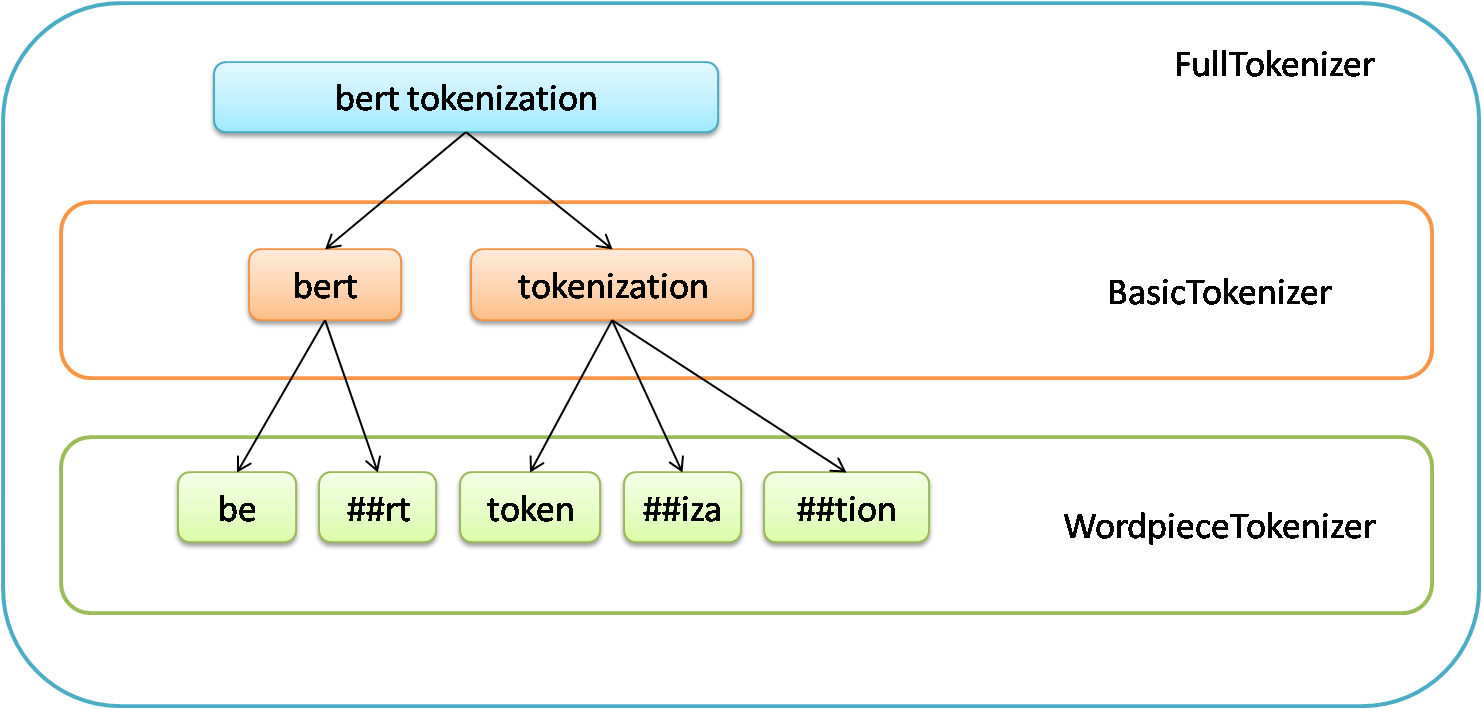
\includegraphics[width=0.8\textwidth]{figs/tokenization.png}}
%                     \caption{نمونه‌ای از کارکرد Tokenizer}
%                     \label{fig:tokenization}
%                 \end{figure}
%         \item  \textbf{بردارهای تصویر:}
%                 برای تبدیل تصاویر به بردارهای ویژگی مطابق با مقاله‌ای برای حل
%                 مسائل زبان-تصویر 
%                 \cite{anderson2018bottom}
%                 می‌توانیم هر تصویر را مجموعا به صورت 36 شیء در نظر بگیریم که از 
%                 شبکه عصبی
%                 \lr{Faster-RCNN} \cite{ren2015faster}
%                 تشخیص داده‌شده و هر شیء برداری با اندازه 2048 دارد.
                            
%     \end{enumerate}
% }

% \section {
%   مدل Encoder
%  }
% \paragraph{}{
%     از آنجایی که در بخش‌های قبل گفته شد، از مدل‌های از پیش آموزش داده‌شده 
%     استفاده می‌کنیم. به منظور مقایسه هر دو حالت تک‌جریان و دوجریان از دو مدل
%     تبدیل شونده با معماری‌های متفاوت استفاده شده است تا بتوان مقایسه جامع و
%     کاملی حول انواع مدل‌ها و عملکرد آن‌ها داشت. هدف از به کارگیری 
%     بخش کدگذار محاسبه یک بازنمایی از پرسش و تصویر همراه با یک‌دیگر و 
%     عبور دادن آن به بخش کدگشا است.
% }

% \subsection {
%   مدل LXMERT \cite{tan-bansal-2019-lxmert}
%  }
% \paragraph{}{
%     این مدل به عنوان یک مدل پایه برای حل مسئله پرسش و پاسخ تصویری ارائه شد. 
%     این مدل شامل سه بخش کدگذار تصویری، زبانی و میان‌ماژولی است. این مدل دو ورودی
%     می‌گیرد، یک تصویر و یک متن که همان پرسش مربوط به تصویر است. با 
%     ترتیب لایه‌های توجه به خود و توجه میانی باعث می‌شود که مدل بتواند 
%     یک بازنمایی از تصویر، یک بازنمایی از متن و یک بازنمایی 
%     میان‌ماژولی از ورودی‌ بدست بیاورد.  محققان در این مدل از روش‌های متفاوتی نظیر 
%     \lr{MLM} \footnote{\lr{Masked Language Modeling}}
%     ، MOP \footnote{\lr{Masked Object Prediction}}
%     و
%     تناظر میان‌ماژولی
%     \footnote{\lr{Cross-modality Matching}}
%     برای 
%     آموزش استفاده کرده‌اند که باعث شده است روابط درون‌ماژولی
%     و میان‌ماژولی به خوبی تشخیص داده شود. همانطوری که از تصویر 
%     \ref{fig:lxmert}
%     مشخص است این مدل یک مدل دوجریان است. 
%     \begin{figure}[H]
%         \center{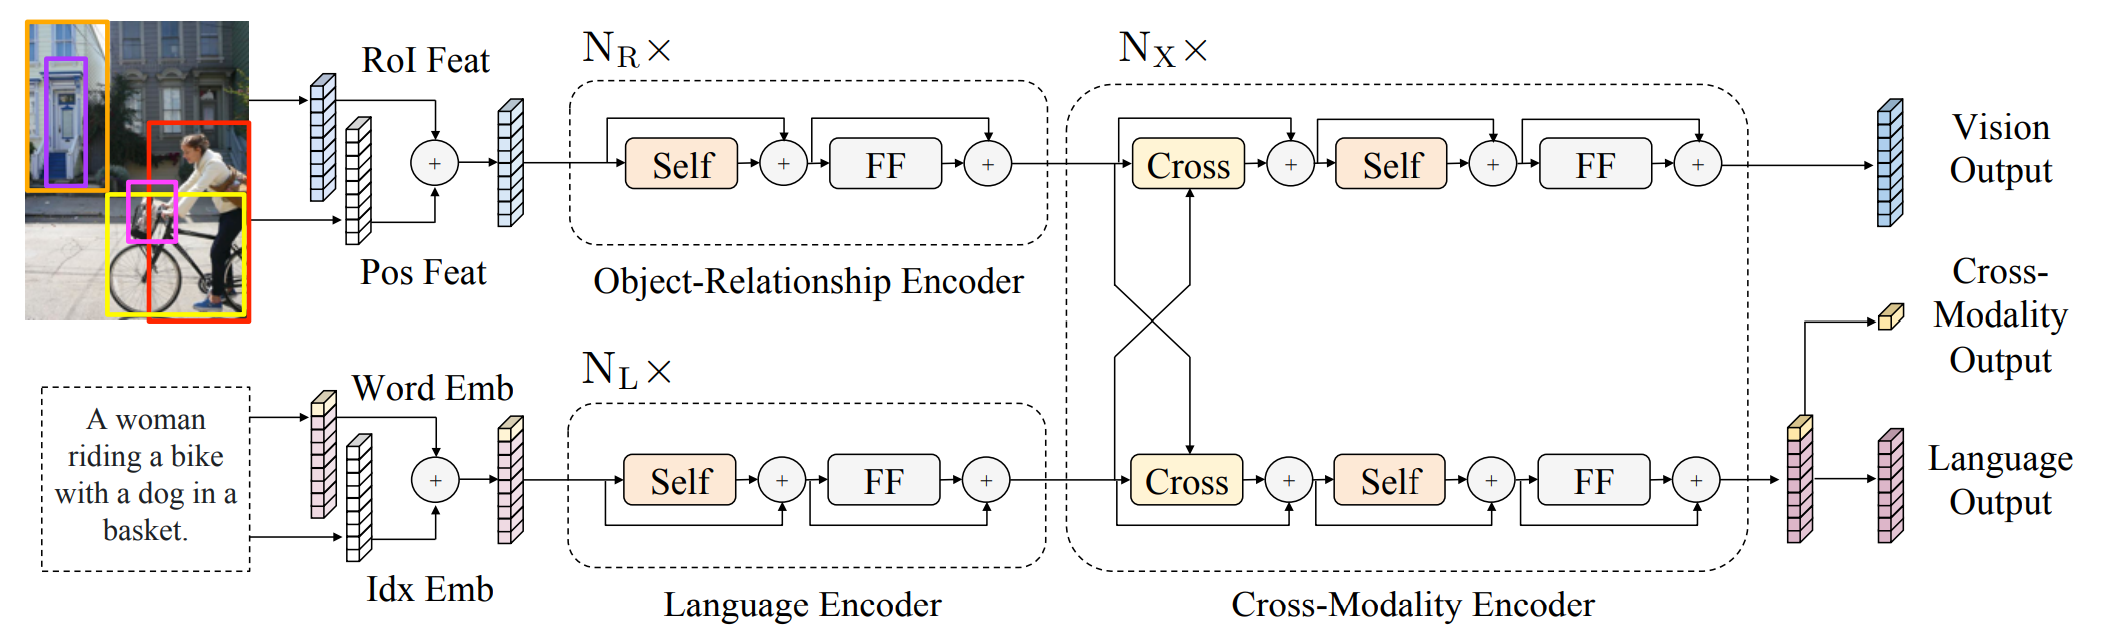
\includegraphics[width=1\textwidth]{figs/lxmert.png}}
%         \caption{معماری مدل LXMERT همراه با ورودی و خروجی}
%         \label{fig:lxmert}
%     \end{figure}
% }

% \subsection{
%     مدل VisualBERT \cite{li-etal-2020-bert-vision}
% }

% \paragraph{}{
%     پس از انتشار 
%     LXMERT
%     و پیشرفت چشمگیرش در حل مسئله پرسش‌وپاسخ تصویری پژوهش‌های بسیاری 
%     برای بهبود بیشتر انجام شد. از جمله این پژوهش‌ها بررسی مدل 
%     BERT
%     و عملکرد آن در مسائل زبان-تصویر را میتوان نام برد که منجر به انتشار مدل
%     VisualBERT \cite{li-etal-2020-bert-vision}
%     شد. این مدل به صورت تک‌جریان است و دنباله‌ای از بردار‌های ویژگی متن
%     همراه با دنباله‌ای از بردارهای ویژگی تصویر را ورودی می‌گیرد و خروجی را
%     به صورت بردارهای بازنمایی می‌دهد. به علاوه، میزان توجه 
%     بردار‌های ویژگی توکن‌ها و بردار‌های ویژگی اشیاء موجود در تصویر 
%     را با یکدیگر اندازه‌گیری کردند و اشیاء با توکن‌های مربوطه به‌خوبی
%     توجه خورده‌اند. برای مثال با توجه به شکل 
%     \ref{fig:visualbert}
%     در لایه 11 کلمه 
%     man
%     به خوبی با محدوده مربوط به مرد موجود در تصویر مرتبط شده است!
%     \begin{figure}[H]
%         \center{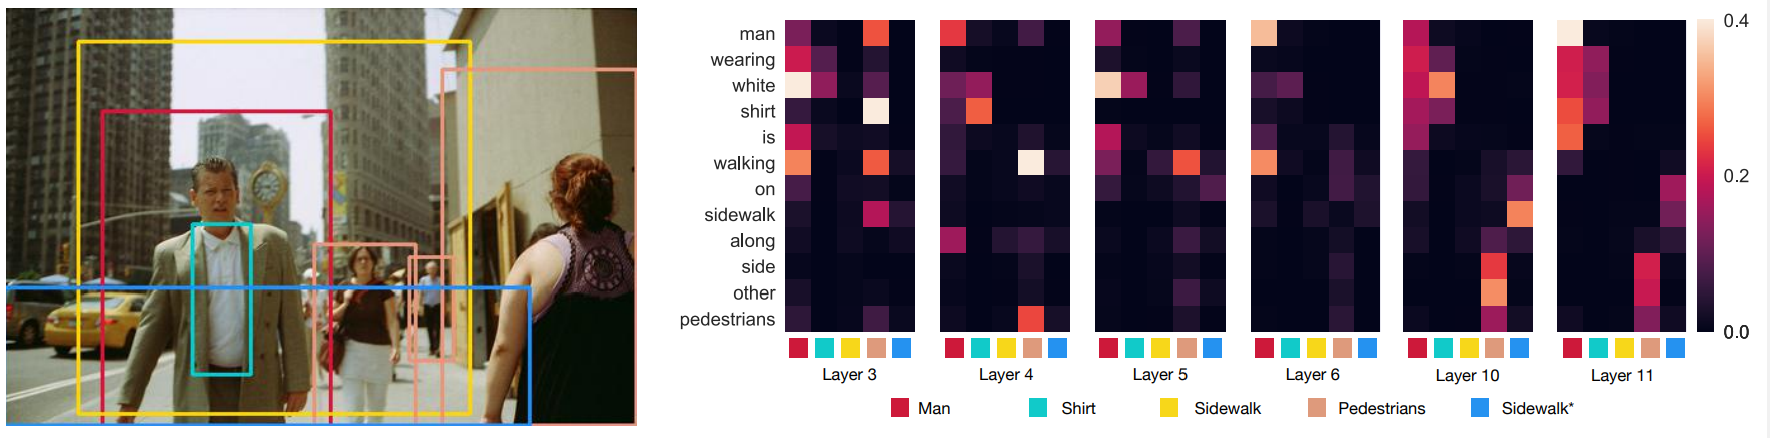
\includegraphics[width=1\textwidth]{figs/VisualBERT.png}}
%         \caption{میزان توجه بخش متن به تصاویر در VisualBERT}
%         \label{fig:visualbert}
%     \end{figure}
% }

% \section{
%   مدل Decoder
%  }
% \paragraph{}{
%     پس از آنکه بردارهای بازنمایی تصویر و پرسش توسط کدگذار محاسبه شد، لازم
%     است که أن‌ها را برای تولید پاسخ به بخش کدگشا بدهیم. 
%     بخش کدگشای معماری‌های ارائه شده از دو معماری شبکه‌های عصبی بازگشتی و 
%     شبکه‌های تبدیل‌شونده استفاده شده است. برای تولید پاسخ از مکانیزم
%     Autoregressive 
%     استفاده شده است. در این مکانیزم توکن‌ها بر اساس توکن‌های قبلی پیش‌بینی می‌شوند
%     و سپس همان توکن جدید همرا با دنباله قبلی برای توکن جدید دیگری مطابق با
%     شکل 
%     \ref{fig:decoder}
%     به کدگشا 
%     ورودی داده می‌شوند. 
%     \begin{figure}[H]
%         \center{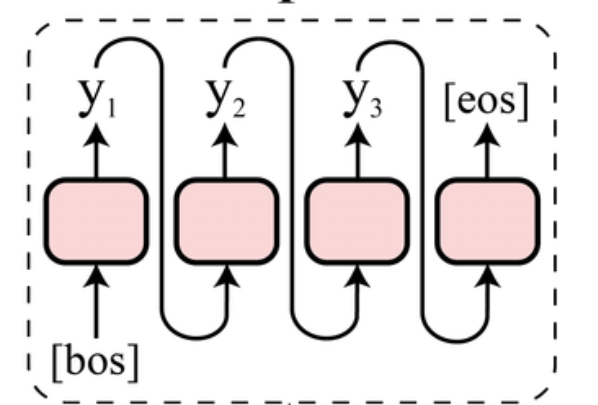
\includegraphics[scale=1]{figs/Autoregressive.png}}
%         \caption{ساختار مدل \lr{Autoregressive Decoder}}
%         \label{fig:decoder}
%     \end{figure}
% }

% \section{جمع‌بندی}
% \paragraph{}{
%     در این بخش از نوشتار به بررسی دقیق اجزای تشکیل‌دهنده‌ی سیستم پیشنهادی برای
%     حل مسا‌له‌ی پرسش‌وپاسخ تصویری پرداختیم.
%     روشی نو برای حل این‌ مسئله که باعث رفع ابهامات بسیاری می‌شود. اشاره شد که
%     از مدل‌های از پیش آموزش داده‌شده استفاده کردیم و همچنین برای 
%     مقایسه نتایج و بدست آوردن بهترین معماری، چندین حالت بررسی شد که در 
%     بخش
%     \ref{ch:eval}
%     به مقایسه نتایح پرداخته‌ خواهد شد.
% }